%%% The main file. It contains definitions of basic parameters and includes all other parts.

%% Settings for single-side (simplex) printing
% Margins: left 40mm, right 25mm, top and bottom 25mm
% (but beware, LaTeX adds 1in implicitly)
\documentclass[12pt,a4paper]{report}
\setlength\textwidth{145mm}
\setlength\textheight{247mm}
\setlength\oddsidemargin{15mm}
\setlength\evensidemargin{15mm}
\setlength\topmargin{0mm}
\setlength\headsep{0mm}
\setlength\headheight{0mm}
% \openright makes the following text appear on a right-hand page
\let\openright=\clearpage

%% Settings for two-sided (duplex) printing
% \documentclass[12pt,a4paper,twoside,openright]{report}
% \setlength\textwidth{145mm}
% \setlength\textheight{247mm}
% \setlength\oddsidemargin{14.2mm}
% \setlength\evensidemargin{0mm}
% \setlength\topmargin{0mm}
% \setlength\headsep{0mm}
% \setlength\headheight{0mm}
% \let\openright=\cleardoublepage

%% Generate PDF/A-2u
\usepackage[a-2u]{pdfx}

%% Character encoding: usually latin2, cp1250 or utf8:
\usepackage[utf8]{inputenc}

%% Prefer Latin Modern fonts
\usepackage{lmodern}

%% Further useful packages (included in most LaTeX distributions)
\usepackage{amsmath}        % extensions for typesetting of math
\usepackage{amsfonts}       % math fonts
\usepackage{amsthm}         % theorems, definitions, etc.
\usepackage{bbding}         % various symbols (squares, asterisks, scissors, ...)
\usepackage{bm}             % boldface symbols (\bm)
\usepackage{graphicx}       % embedding of pictures
\usepackage{fancyvrb}       % improved verbatim environment
\usepackage{natbib}         % citation style AUTHOR (YEAR), or AUTHOR [NUMBER]
\usepackage[nottoc]{tocbibind} % makes sure that bibliography and the lists
			    % of figures/tables are included in the table
			    % of contents
\usepackage{dcolumn}        % improved alignment of table columns
\usepackage{booktabs}       % improved horizontal lines in tables
\usepackage{paralist}       % improved enumerate and itemize
\usepackage{xcolor}  % typesetting in color

%% Additional packages
\usepackage{amsthm}
\usepackage[allow-number-unit-breaks, detect-all]{siunitx}
\usepackage{textcomp}
\usepackage[acronym]{glossaries}
\usepackage{fancyvrb}
\usepackage{enumitem}
\usepackage{mathtools}
\usepackage{interval}
\usepackage{cprotect}
\usepackage{todonotes}
\usepackage{graphicx}
\usepackage{caption}
\usepackage{subcaption}
\usepackage{nicefrac}
\usepackage{url}
\usepackage{float}
\usepackage{tikz}
\usetikzlibrary{calc}
\usetikzlibrary{scopes}
\usetikzlibrary{intersections}
\usetikzlibrary{quotes,angles}
\usepackage{tabularx}

%% Algorithms (https://www.overleaf.com/learn/latex/algorithms)
\usepackage[linesnumbered,algoruled,boxed,lined]{algorithm2e}
\SetKwComment{Comment}{$\triangleright$\ }{}
\SetKwInOut{Parameter}{Parameter}
\SetKw{Continue}{continue}

%% Custom settings
\renewcommand\vec{\bm}
\VerbatimFootnotes
\newcommand\norm[1]{\left\lVert#1\right\rVert}
\DeclareMathOperator*{\argmin}{arg\,min} % Jan Hlavacek
\DeclareMathOperator*{\argmax}{arg\,max}
\DeclareMathOperator{\sign}{sgn}
\newcommand{\bftab}{\fontseries{b}\selectfont}

%% Glossaries
\makeglossaries

\newacronym{AMCL}{AMCL}{Adaptive Monte Carlo Localization}
\newacronym{ROS}{ROS}{Robot Operating System}
\newacronym{EKF}{EKF}{Extended Kalmann Filter}
\newglossaryentry{LIDAR}{name={LIDAR},description={Light Detection And Ranging}}
\newglossaryentry{PID}{name={PID},description={Proportional-integral-derivative controller}}
\newacronym{IMU}{IMU}{Inertial Measurement Unit}
\newacronym{PWM}{PWM}{Pulse Width Modulation}
\newacronym{ESC}{ESC}{Electronic Speed Controller}
\newacronym{RC}{RC}{Radio-controlled}
\newacronym{DC}{DC}{Direct Current}
\newacronym{SLAM}{SLAM}{Simultaneous Localization And Mapping}
\newacronym{REP}{REP}{ROS Enhancement Proposal}
\newacronym{DWA}{DWA}{Dynamic Window Approach}
\newacronym{RPM}{RPM}{Revolutions Per Minute}
\newacronym{RRT}{RRT}{Rapidly-Exploring Random Trees}
\newacronym{RRT*}{RRT$^*$}{Optimal RRT}
\newacronym{SEHS}{SEHS}{Space Exploration Guided Heuristic Search}

%%% Basic information on the thesis

% Thesis title in English (exactly as in the formal assignment)
\def\ThesisTitle{Trajectory planning for fast moving cars}

% Author of the thesis
\def\ThesisAuthor{Šimon Rozsíval}

% Year when the thesis is submitted
\def\YearSubmitted{2020}

% Name of the department or institute, where the work was officially assigned
% (according to the Organizational Structure of MFF UK in English,
% or a full name of a department outside MFF)
\def\Department{Department of Theoretical Computer Science and Mathematical Logic}

% Is it a department (katedra), or an institute (ústav)?
\def\DeptType{Department of Theoretical Computer Science and Mathematical Logic}

% Thesis supervisor: name, surname and titles
\def\Supervisor{Prof. RNDr. Roman Barták, Ph.D.}

% Supervisor's department (again according to Organizational structure of MFF)
\def\SupervisorsDepartment{Department of Theoretical Computer Science and Mathematical Logic}

% Study programme and specialization
\def\StudyProgramme{Computer Science}
\def\StudyBranch{Artificial Intelligence}

% An optional dedication: you can thank whomever you wish (your supervisor,
% consultant, a person who lent the software, etc.)
%\def\Dedication{%
%Dedication.
%}

% Abstract (recommended length around 80-200 words; this is not a copy of your thesis assignment!)
\def\Abstract{%
The goal of this thesis is to create an artificial agent for an autonomous racing vehicle.  This project is inspired by the F1/10 racing competition. The agent uses a planning algorithm to find a time-optimal trajectory. To achieve real-time performance, the agent analyzes the map of the track and it focuses only on the next two corners immediately ahead of the vehicle. The agent replans the trajectory several times per second to adjust the trajectory to the inherently imperfect trajectory following. We successfully tested the agent in a simulator with good results. We also tested the algorithm on a custom car-like robot equipped with an on-board computer and sensors, but with limited success.
}

% 3 to 5 keywords (recommended), each enclosed in curly braces
\def\Keywords{%
{planning}, {autonomous vehicle}, {autonomous racing}
}

%% The hyperref package for clickable links in PDF and also for storing
%% metadata to PDF (including the table of contents).
%% Most settings are pre-set by the pdfx package.
\hypersetup{unicode}
\hypersetup{breaklinks=true}

% Definitions of macros (see description inside)
\include{macros}

% Title page and various mandatory informational pages
\begin{document}
\include{title}

%%% A page with automatically generated table of contents of the master thesis

\tableofcontents

\listoftodos

%%% Each chapter is kept in a separate file
\chapter*{Introduction}
\addcontentsline{toc}{chapter}{Introduction}

Autonomous vehicles are slowly making their way from research facilities to the public roads around the world and it seems inevitable that soon they will become parts of our everyday lives. Autonomous vehicles could have great impact on transportation of people and goods. For example, thousands of people die in car accidents every year because of human error \cite{Road_accidents}. Some believe that replacing humans with accurate electronic sensors and computer algorithms, which never make errors, could reduce the number of accidents on roads significantly. It seems that companies around the world see the potential in this technology and invest a lot of effort and money in research of self-driving cars. Even though nobody can guarantee that autonomous vehicles will never make errors and that they will solve other problems of road transportation we face today, the trend seems to be clear. The key to the success of this technology will be reliable and robust algorithms which will work in all driving scenarios and weather conditions and which the public will trust. 

The idea of self-driving cars is not a new one. Prototypes of autonomous vehicles were demonstrated on public roads already in the 1980s. Some of the well-known projects from this era were for example the NavLab vehicle of the Carnegie Mellon University \cite{NavLab} or the project of Ernst Dickmanns in cooperation with the Daimler company \cite{Ernst_Dickmanns}. The DARPA challenges, organized between 2004 and 2007, gained a lot of media attention. We could see that self-driving cars are not just sci-fi anymore. Since then, many driving assistants such as adaptive cruise control, lane keeping assistants, parallel parking assistants and collision warning and emergency braking assistants started appearing in commercially available vehicles. Some systems, like the Tesla Autopilot, go even further and allow complex autonomous maneuvers such as overtaking of other vehicles.

These commercially available assistants provide only partial autonomy. They require the driver to always pay attention to the road and to be prepared to take over the control of the vehicle. Fully autonomous vehicles will not require any human interaction and they might even lack any means of manual driving input and they might not even have a steering wheel and the pedals. The computer will be responsible for the vehicle from the start to the destination no matter what the weather and traffic is like outside. There is an ongoing research into full autonomy by some companies, including Waymo and Uber, and the prototypes of these vehicles are already being tested on public roads.

One of the key problems in autonomous driving is the ability to find a good trajectory for the car. This trajectory must be safe for the passengers of the vehicle and for other road users. It must also conform to road limitations such as speed limits and other traffic rules. Automated planning is an area of artificial intelligence which gives us means to solve this problem. For a well-defined planning problem which describes the physics of the vehicle and what our goals are, we can find a sequence of control inputs for the given type of vehicle which will drive the vehicle the way we need.

The goal of this thesis is to create an artificial agent which will autonomously drive along a racing circuit utilizing a trajectory planning algorithm. The agent must avoid any collision with the boundary of the track or any static obstacles on the track while trying to achieve fast lap times. We will not consider the option of head-to-head racing where there are multiple competing cars moving on the track at the same time and all the obstacles on the track will be stationary.

We will formulate a trajectory planning problem of driving through a series of waypoints while aiming for fast lap times. This thesis explores ways of finding a solution to this problem with a knowledge of an approximate model of the vehicle. Alongside the planning algorithm, we explore the possibilities of following the selected reference trajectory as closely as possible while avoiding obstacles which were not known at the time of planning. These two algorithms are combined in an autonomous racing agent which uses the trajectory planning algorithm to find a trajectory for the next few corners ahead, and then follows this trajectory. We implement and test this racing behavior on a 1:10 scale car-like robot with a set of on-board sensors and an embedded computer.

First, we introduce the autonomous driving problem and split it into several sub-problems. We give a brief overview of related works in the field of autonomous driving.

Next, we examine how the vehicle reacts to steering commands and we describe two vehicle models with different levels of complexity and accuracy in the chapter Vehicle Model. With a model of the vehicle defined, we formulate the trajectory planning problem for an autonomous racing car, and we describe several methods of finding a feasible plan in the chapter Trajectory Planning Problem. The chapters Trajectory Following and The Racing Agent then combine the previously described algorithms into the final autonomous racing agent.

Finally, we implement the racing agent and we conduct several experiments to verify the performance and success rate of our algorithms on a physical robot in the chapter Experimental Verification, and summarize our findings.

\chapter{Autonomous Driving Background}

Autonomous driving is a complex task. The vehicle collects information about the surrounding environment from its sensors and then it decides its next control input to the actuators of the vehicle. There are two general approaches to this problem: end-to-end driving and decomposition into several subproblems.

The end-to-end driving approach takes the sensor data as an input and maps them to the control inputs. The end-to-end driving algorithm can be implemented for example using a stream of images form a front-facing camera and a neural network trained using supervised or reinforcement learning. It was successfully demonstrated for example in ALVINN, a simple 3-layer neutral network used in the NavLab autonomous vehicle of Carnegie Mellon University in 1989 \cite{ALVINN}, or more recently with a deep convolutional neural network by Nvidia \cite{Nvidia}. End-to-end driving avoids explicit modeling of the world and the vehicle and it relies on the knowledge extracted from the training data or by learning by trial and error during reinforcement learning.

The other approach is to split the complex problem into several smaller problems, which are solved independently. We can split the problem into three main subproblems: Perception, Planning, and Control.

Perception is the process of collecting data from the sensors and processing them to obtain the current state of the world and the internal properties of the vehicle. The task of determining the position of the vehicle on a map is called localization. The sensors which would be used for localization are cameras, radars, ultrasonic sensors, and LIDARs. The data from these sensors can be used to determine distances to nearby obstacles in different directions. Based on the previous known position of the vehicle, the estimate of its movement, and the distances to obstacles in different directions, the position on a known map can be determined using an algorithm such as Adaptive Monte Carlo Localization (AMCL) \cite{AMCL_position_estimation} \cite{AMCL_adaptive_sampling}. In certain scenarios, the relative distances to the obstacles might not be enough to determine correct position. This can happen for example when the vehicle is driving through a straight tunnel and the distances to the walls are constant even though the vehicle is moving. It is useful to combine readings from multiple sensors which provide odometry such as wheel encoders which measure how many times the wheels turn and an intrinsic measurement unit (IMU) with gyroscopes and accelerometers which measures the linear and angular acceleration of the vehicle. The combination of multiple different types of sensors is called sensor fusion. Kalman filter is an example of an algorithm which is frequently used to fuse data from different sources \cite{Kalman_filter}.

The vehicle must also be able to read road signs and road surface markings for driving along public roads. The data from the sensors can also be used to detect obstacles and for obstacle tracking. The type of obstacle is then identified and in the case of dynamic obstacles such as other cars, bicyclists, pedestrians, animals, or moving inanimate objects their movement in time must be predicted to prevent collisions.

The geometry of a car-like vehicle limits its controllability. The vehicle cannot turn while it is stopped and it can only start turning once it is moving forwards or backwards. Usually the only way to control the turning radius is by turning the front wheels and the rear wheels are fixed. In order to be able to make any reasoning about the future states of the vehicle, we must be able to predict the effect of a sequence of control inputs on the motion of the vehicle. Without an accurate model of the vehicle we could select a trajectory which cannot be safely followed, or which would be ineffective. We will discuss vehicle modelling in detail in chapter Vehicle Model.

With the knowledge of the vehicle model, we can search for a plan consisting of control inputs over some time period which will result in a collision-free trajectory through the environment which minimizes some cost function (e.g., the time it will take to reach some goal location). Planning several steps into the future can give us an advantage over a simple end-to-end driving approach. For example, in the case of autonomous racing, the agent can take advantage of the knowledge of the racing track map, and account for the shape of the track hidden around the next corner. We should be able to decide, when to slow down and when to accelerate, as well as at which point to start turning into a corner, in order to reach the best lap times. We call this subproblem trajectory planning.

Executing the sequence of control inputs one by one might cause the vehicle to drive off the track. The trajectory planning algorithm relies on a vehicle model which might not be accurate. The reference trajectory is therefore idealized, and it might not be possible to achieve it exactly by the actual vehicle. It might also lead to a collision with an obstacle on the track which was not known at the time of planning. A trajectory following algorithm chooses the next action based on the current state of the vehicle and the distance to the position, vehicle orientation, and speed at a corresponding point on the reference trajectory. The algorithm should also avoid any unexpected obstacles detected by the sensors.

The actual effects of the control inputs are measured by the sensors and the control algorithm tries to minimize the error between the planned trajectory and the actual trajectory of the vehicle in its next step. This process is referred to in control theory as closed feedback loop.

\section{Requirements}

In this thesis, we will design and develop an autonomous vehicle for the task of autonomous racing. The racing scenario is a simplification of real-world driving. It requires us to avoid collisions and to find efficient trajectories while moving at high speeds and to adapt to unforeseen obstacles on the road. At the same time, this relaxed problem allows us to ignore any traffic rules. We do not have to consider any speed limits, crossroads, or stop signs.

This problem is inspired by the F1/10 competition organized by the University of Pennsylvania and the University of Virginia \cite{F1/10_web}. We will use the resources from this competition to build a similar autonomous vehicle based on an RC car. To evaluate the performance of the vehicle, we will use the criteria of Time Trial Race of F1/10. In the Time Trial Race, the vehicle drives for 5 minutes around a circuit trying to achieve as many laps as possible without a collision with the boundary of the track or with static obstacles on the track. The time of the fastest lap is also recorded.

We will create an autonomous racing agent which utilizes a trajectory planning algorithm to find fast routes along the racing circuit. We will test different algorithms for searching solutions to the planning problem and compare them in a series of experiments on a real-world car model with sensors and an embedded on-board computer.

\section{Related Work}

In this section we will go through several interesting approaches to path and trajectory planning from the area of robotics and autonomous cars.

Shakey the Robot was a project at the Stanford Research Institute in the 1960s. For the purposes of efficient route finding the A* algorithm was designed by Nils J. Nilsson and his coworkers \cite{Nilsson}. This algorithm is widely used for solving various graph search problems thanks to its simplicity, completeness, and optimality. The NavLab autonomous vans of the Carnegie Mellon university was one of the first autonomous vehicles tested on public roads in the 1980s and 1990s. One of the interesting results of their work is the Pure Pursuit control algorithm \cite{Pure_pursuit}.

Steven M. LaValle designed a randomized path planning algorithm for vehicles with kinodynamic driving constraints and high-dimensional configuration spaces called Rapidly-Exploring Random Trees (RRT) \cite{RRT}. This algorithm randomly samples the configuration space and steers the vehicle towards the sampled point in the space. A tree of feasible paths in the configuration space rooted in the starting position is constructed until a path which ends in the goal position is found. The algorithm is probabilistically complete, but it is not optimal. The algorithm was extended by many times in order to converge faster and to be optimal. The optimal variant of the algorithm, RRT* \cite{RRT_star}, is unfortunately hard to use for car-like vehicles.

In 2007, the DARPA Urban Challenge took place in the USA which was successfully completed by several vehicles with different approaches to trajectory planning. The entry from the Carnegie Mellon University, Boss, won the competition. It uses the Anytime D* algorithm for navigation in unstructured environment \cite{Boss}. The Stanford team used an algorithm called Hybrid A* in their vehicle called Junior \cite{Junior}. This algorithm is an extension of the A* algorithm which discretizes the continuous search space into a discrete grid to avoid examining similar configurations multiple times, but it keeps the information about the trajectories in the continuous configuration space to produce smooth feasible trajectories. The team from MIT used modified RRT algorithm in their vehicle \cite{RRT_urban_driving}.

\chapter{Artificial Racing Agent}

In this chapter we will first analyze how human racing drivers approach the task of car racing. We will then use this information to design a behavior of an autonomous agent and decompose the problem into several smaller tasks. We will discuss how we can analyze the racing track and prepare it for trajectory planning.

\section{Racing Line}

When a human driver drives on a racing circuit, his or her task is to complete several laps around the circuit in a time period as short as possible. In order to minimize the lap times, the driver trades off the total distance the car travels for the average speed at which it moves. The trajectory of the vehicle through the racing track is sometimes referred to as the racing line and it depends on the shape of the track and on the vehicle. The driver will follow different racing lines for different vehicles on the same circuit based on many their different properties such as maximum speeds, acceleration, braking power, or the grip of the tires.

For a turn with a steady curvature there is a maximum speed at which a specific car can go and stay on the track. Exceeding this speed will cause a loss of friction between the tires and the road surface and the tires will not be able to exert enough lateral force to keep the car on the curve and the car will start to travel along a curve with a greater radius than the one commanded by the driver. This situation is called understeer or oversteer, depending on whether it was the front or rear wheels which lost the friction and which wheels are powered by the engine.

% todo: image of oversteer and understeer

On the other hand, for a constant vehicle speed, the vehicle can safely travel along any curve with a radius greater than the minimum safe radius. The driver will therefore try to follow curves with higher radii when going through corners but only to the point where the maximum safe speed reaches the maximum speed of the vehicle. Increasing the curvature when it is not possible to increase the speed adds to the distance the car travels but it does not increase the average speed and therefore leads to a higher lap time.

The trajectory of the vehicle as it goes through a corner can be split into several stages. First, the vehicle aligns itself to the outer edge of the track. Second, the vehicle must adjust its speed so it can safely stay on the curve. It is common to use the brakes mostly while the vehicle is moving straight to avoid locking the wheels in mid-turn. Third, the car starts turning at a turn-in point to go through the apex of the curve at the desired moment. Fourth, the vehicle goes through an apex, which is the point, where it is the closest to the inner edge of the track. Next, the vehicle starts exiting the corner and enters another part of the track.

There are two common ways of going through a corner, a classical one and one called late apex. The classical way of leaving the corner is to keep the constant curvature of the turn and to align the vehicle with the outer edge of the track. The late apex is achieved by starting to turn into the corner later and exiting the corner much closer to the inner edge of the track than the classical way. During the late apex turn, the vehicle slows down more before entering the corner and it straightens the line before hitting the apex allowing for greater exit speed. The comparison between these two lines can be seen in **todo figure**.

% figures to use: https://drivingfast.net/racing-line/#chapter-1

Another factor which affects the speed at which the driver can go through a corner is the shape of the track around the corner. When there is a straight stretch following the corner, the driver can maximize the speed at which the vehicle leaves the corner to increase the average speed. If there is another corner immediately after the first one, the driver must plan ahead and adjust the speed before entering the first corner to a level at which the exit speed of the first corner will be appropriate to go through the following corner.

From the description of the racing behavior of human expert drivers, it is apparent that the key components of choosing the optimal racing line are the knowledge of the behavior of the vehicle and the shape of the track. The knowledge of the track gives the driver an opportunity to plan how he or she is going to approach driving on the track. The driver can plan how to approach each individual corner and what speeds and turning radii are optimal and still safe.

\section{Artificial Agent}

\begin{defn}\label{def:rational_agent}
    A rational agent is an entity which gathers information from the environment through sensors and changes the state of the environment in order to maximize some performance measure.
\end{defn}

A racing driver can be thought of as a rational agent as defined in definition~\ref{def:rational_agent}. The driver observes the position of the vehicle on the racing track and the state of the vehicle as it moves along the track. He also observes the distance to the boundaries of the track and to any obstacles which can be present on the track. The driver reacts to these perceptions by giving control inputs to the vehicle through the steering wheel, brake and accelerator pedals, and shifting into different gears. The performance measure is the lack of collisions with the boundaries of the track or any obstacles on the track and minimizing of the lap time.

An artificial racing agent would use electronic sensors such a LIDAR, wheel encoders, an IMU, or a camera to observe the state of the environment. Based on this observation, the agent can estimate its state in the world and the state of other entities in the world, such as obstacles or opponents. Based on this information, the agent has to select a control input for the actuators of the vehicle.

The agent can use the information about its initial state and calculate a time-optimal racing line from this initial state through the whole circuit up to the finish line using a trajectory planning algorithm. Depending on the size of the circuit, this could be a computationally expensive operation. If later on there is a need to re-plan the trajectory during the race, because the vehicle could not follow the trajectory accurately and it is necessary to come up with a contingency plan, the vehicle might have to repeat the expensive calculation. Instead, the agent can analyze the shape of the circuit and identify the corners and focus its effort only on the next two or three corners ahead of him.

\subsection{Decision Process}

An agent is sometimes described in the form of an agent function. This function takes the data from the sensors and outputs a command for the actuators. The command is then executed and it has an effect on the environment. In the next step we measure the changed state of the environment and the agent reacts to this changed state. The agent can select the next command in an order to correct the outcome of the previous command when it is different from the predicted outcome. This process is then repeated over and over in a so-called closed-feedback loop.

In order to avoid describing the logic of the racing agent in a single complicated function, we can divide the decision process of the agent into several smaller independent sub-problems: localization, track analysis and waypoint selection, trajectory planning, and trajectory following. Some of these sub-problems output information which is necessary as an input for another of these sub-problems they form nodes of a dependency graph of the decision process which is visualized in Figure~\ref{fig:racing_agent_diagram}.

There is one more reason to decompose the task into independent subproblems. The rate at which the nodes produce outputs is different and they work asynchronously. While the trajectory following node should react to any location update with an action to correct the movement of the vehicle and it should do this many times per second, the planning process of a trajectory will take some non-trivial time and so the trajectory planning node will have much lower output frequency.

\begin{figure}[]\centering
\includegraphics[width=125mm]{../img/racing_agent_diagram.pdf}
\caption{A diagram of the decision process of the racing agent.}
\label{fig:racing_agent_diagram}
\end{figure}

\paragraph{Track analysis} Before the race begins, the agent analyses the track and finds the corners and bends on the track and marks a coordinate of a point near the apex of the corner. This analysis will give us the opportunity to focus the planning effort only to driving through the next few corners directly ahead of of the agent.

\paragraph{Vehicle model} Vehicle modeling is also a separate problem. The description of the behavior of the vehicle with a set of differential equations is key to a successful planning of feasible trajectories and for accurate trajectory following.

\paragraph{Localization} As the vehicle moves on the track, the agent needs to know its current position, orientation, and speed. A localization algorithm collects the data from different sensors and estimates the current state of the vehicle. The accuracy and the frequency of state updates depend greatly on the capabilities of the sensors and the processing power of the on-board computer. The responsibility of the localization algorithm is to publishes the vehicle state updates as frequently as possible and without a long delay between the time at which the data came from the sensors and at which it will be used as an input for trajectory planning and trajectory following.

\paragraph{Waypoint selection} During the race, the agent will keep track of which of the waypoints discovered during track analysis it drove past the last. The waypoint selection node will publish the following $n$ waypoints as the next goal for trajectory planning. The parameter $n\in\mathbb{N}$ is the lookahead of the agent. The selection of this parameter is a trade off between the quality of the trajectory and the size of the configuration space that will be search. This directly affects the update rate of the trajectory planning node.

\paragraph{Trajectory planning} The trajectory planning algorithm finds a feasible trajectory from the last state of the vehicle estimated by the localization node through the selected waypoints. The trajectory planning node will start planning a new trajectory as soon as it finishes planning the previous one. As the agent drives along the circuit and drives past a waypoint, the trajectory planning algorithm receives a new sequence of waypoints and the next trajectory it plans will account also for the next corner of the circuit within the lookahead instance. Planning can be a slow process even when we try to reduce the size of the search space as much as possible. For the practical application, the planning algorithm must update the trajectories faster than the vehicle moves through the circuit. If the agent comes to the end of an old reference trajectory and it has no update, it has to stop and wait for an update. This would obviously affect the lap time which is undesirable.

\paragraph{Trajectory following} The latest reference trajectory and the current estimate of the state of the vehicle is used to calculate the next command for the actuators of the vehicle. In the ideal case, this trajectory following node will send the commands to the hardware at the maximum possible rate which the hardware is capable of. In practice we are limited by the rate at which we receive the state estimates from the localization node. The trajectory following node is also responsible for collision avoidance either by actively guiding the vehicle around the obstacles it might hit, or by slowing down the vehicle while waiting for a new reference trajectory.

\subsection{Track Analysis}

The definition of a racing circuit is given by an occupancy grid, initial coordinates of the vehicle in the grid and its heading direction, and at least two more checkpoints which define the direction in which the agent must drive along the circuit. An occupancy grid can be formalized with the following definition:

\begin{defn}\label{def:occupancy_grid}
    Occupancy grid $G\in\{0, 1\}^{m\times n}$ of resolution $r\in\mathbb{R}$ is a two dimensional table of $m$ rows and $n$ columns which corresponds to a rectangular area of the environment of the width of $m * r$ meters and the length of $n * r$ meters. The cells of the table fill the area as square tiles of the side length of $r$ meters. The value of a cell $G_{ij}$ reflects on the state of its corresponding area:
    
\[   
G_{ij} = 
     \begin{cases}
       0\text{,} &\quad\text{if } i < 0 \vee j < 0 \vee i \geq m \vee j \geq n\\
       0\text{,} &\quad\text{if the corresponding tile contains an obstacle} \\
       1\text{,} &\quad\text{otherwise.}
     \end{cases}
\]
\end{defn}

The goal of the track analysis algorithm is to find interesting points of the track which split the track into smaller segments corresponding to stretches between the corners of the track. It would be hard to define how a corner and its apex look like in an occupancy grid, but we can make a simple observation and derive a simple algorithm which will produce good approximate solutions. We can inflate imaginary rubber walls with the thickness of a given safety radius of the vehicle along the edges of the track and loosely lay an imaginary string through the whole circuit. We can then start tightening the string and eventually it will take a form of alternating straight segments and parts, where it touches the rubber wall at an inner edge of a corner of a track. We can then remove the imaginary rubber walls and start walking along the string starting at the initial position of the vehicle. We will mark the furthest point which is directly visible from the place where we're standing. We will then imaginary walk to this point and repeat the process, until we can see the first point we marked. By directly visible we mean that it is possible to draw a line between the two points in the occupancy grid and it will not intersect a cell containing an obstacle between the two points. This thought process is visualized in figure~\ref{fig:thought_process} on different track layouts.

% figure with the analysis of the track

We will implement this process with a two step algorithm which will identify the apexes of corners and points along long winding bends. The first step will be to find the shortest path through the grid which starts at the initial position of the vehicle, and which goes through the checkpoints in the correct order and at any point it does not come closer to an obstacle than to a distance of the safety radius. The second step will simply traverse the path once and select a subsequence of the points such that for two consecutive points $A$ and $B$, $B$ was the last point of the points immediately following $A$ on the original track which are directly visible from $A$.

The shortest path can be found in several different ways. The simplest approach would be to use a simple grid search on the occupancy grid. An interesting alternative is the Space Exploration algorithm described by Chao Chen \cite{SEHS} which uses a search algorithm to explore the grid using circles of variable radii which depend on the distance to the closest obstacle. The expansion of a circle is achieved by calculating $k\in\mathbb{N}$ points on the circumference of the expanded circle and calculating maximum possible a radius for the given point as a distance to the closest obstacle. We will add the child circle to the open set if its radius is larger than some minimum radius (i.e., we will avoid points too close to obstacles) and if the circle has not been closed yet. A circle will be considered closed if the center of the circle lies inside of an already closed circle. This allows us to avoid exploring some regions of the occupancy grid multiple times. To search the space efficiently, we will use the A* algorithm as the search method. The cost to come to a circle will equal to the distance travelled from the initial position to the circle and the estimate of the cost to go will be equal to the euclidean distance to the goal position. We will stop searching at the moment when we expand a circle which contains the goal position. The outline of the algorithm is described in Algorithm~\ref{alg:space_exploration} and a visualization of the algorithm is shown in Figure~\ref{fig:sehs_space_exploration}.

\vspace{1cm}
\begin{algorithm}[H]
    \SetAlgoLined
    \DontPrintSemicolon
    
    \SetKwFunction{Top}{Top}
    \SetKwFunction{MaxRadius}{MaxRadius}
    \SetKwFunction{PointsOnCircumference}{PointsOnCircumference}
    \SetKwFunction{ReconstructPath}{ReconstructPath}

    \KwIn{Occupancy grid $G$, starting position $\vec{x}_0$, goal position $\vec{g}$}
    \KwOut{Sequence of circles}
    \Parameter{Number of expanded children $k$, minimum radius $r_{min}$}
    
    $r_0\gets$ \MaxRadius{$G$, $\vec{x}_0$}\;
    $O\gets\{(\vec{x}_0, r_0)\}$ \Comment*[r]{Open set}
    $C\gets\emptyset$ \Comment*[r]{Closed set}
    $P\gets\emptyset$ \Comment*[r]{Set of transitions}
    
    \While{$O \neq \emptyset$}{
        $(\vec{x}, r)\gets $\Top{$O$}\;
        $O\gets O\setminus\{(\vec{x}, r)\}$\;

        \If{$\|\vec{x} - \vec{g}\| \leq r$}{
            \KwRet \ReconstructPath{$(\vec{x}, r)$, $P$}\;
        }

        \For{$\vec{p'}$ in \PointsOnCircumference{$(\vec{x}, r)$, $k$}}{
            $r'\gets$ \MaxRadius{$G$, $\vec{p'}$}\;

            \If{$r'\geq r_{min}\ \wedge\ \not\exists (\vec{x_{c}, r_{c}})\in C: \|\vec{x_c} - \vec{p'}\| \leq r_c)$}{
                $O\gets O\cup \{(\vec{p'}, r')\}$\;
                $P\gets P\cup \{\big((\vec{x}, r), (\vec{p'}, r')\big)\}$\;
            }
        }

        $C\gets C\cup\{(\vec{x}, r)\}$\;
    }

    \caption{Space Exploration}
    \label{alg:space_exploration}
\end{algorithm}
\vspace{1cm}

To find the path from the initial position through the check points and to the finish line position, we will simply find the path from the initial point to the first checkpoint and then starting from the last circle of the previous path to the next check point. We repeat this until we close the circuit by reaching the initial position again. The path of circles we find might not be optimal. We can further improve it by iterating over the path it and smoothing it as shown in algorithm~\ref{alg:sehs_smoothing}.

With the path of circles around the circuit, we can now proceed the second step of finding the corners of the circuit. We will traverse the path and mark the centers of circles which are the last directly visible points from the previous point as shown in algorithm~\ref{alg:find_apexes}

\vspace{1cm}
\begin{algorithm}[H]
    \caption{Waypoint Selection}
    \label{alg:find_apexes}

    \SetAlgoLined
    \DontPrintSemicolon
    
    \SetKwFunction{AreDirectlyVisible}{AreDirectlyVisible}

    \KwIn{Occupancy grid $G$, sequence of $n$ points $(\vec{x_i})_{i=0}^{n}$}
    \KwOut{Sequence of points}
    
    $r_0\gets$ \MaxRadius{$G$, $\vec{x}_0$}\;
    $O\gets\{(\vec{x}_0, r_0)\}$ \Comment*[r]{Open set}
    $C\gets\emptyset$ \Comment*[r]{Closed set}
    $P\gets\emptyset$ \Comment*[r]{Set of transitions}
    
    \While{$O \neq \emptyset$}{
        $(\vec{x}, r)\gets $\Top{$O$}\;
        $O\gets O\setminus\{(\vec{x}, r)\}$\;

        \If{$\|\vec{x} - \vec{g}\| \leq r$}{
            \KwRet \ReconstructPath{$(\vec{x}, r)$, $P$}\;
        }

        \For{$\vec{p'}$ in \PointsOnCircumference{$(\vec{x}, r)$, $k$}}{
            $r'\gets$ \MaxRadius{$G$, $\vec{p'}$}\;

            \If{$r'\geq r_{min}\ \wedge\ \not\exists (\vec{x_{c}, r_{c}})\in C: \|\vec{x_c} - \vec{p'}\| \leq r_c)$}{
                $O\gets O\cup \{(\vec{p'}, r')\}$\;
                $P\gets P\cup \{\big((\vec{x}, r), (\vec{p'}, r')\big)\}$\;
            }
        }

        $C\gets C\cup\{(\vec{x}, r)\}$\;
    }
\end{algorithm}
\vspace{1cm}

% todo algorithm smoothing out

% do I need to prove 


\chapter{Trajectory Planning}

The main focus of this thesis is the problem of trajectory planning for a fast moving car. In this chapter, we will analyze this problem in depth. We will first look into the planning problem in general and then we will discuss what the term ``fast moving cars'' means and how trajectory planning for a fast car is different from the general planing problem.

With the knowledge of the theory, we will formulate our trajectory planning problem. We will consider several well-known search algorithms used to solve planning problems and adapt them to our problem.

The solution of the planning problem will be a trajectory. A trajectory is the description of both a path the vehicle should follow and also a speed profile. If a robot is able to follow this trajectory, it will have an advantage over reactive steering algorithms, such as end-to-end driving, as it will be able to go through a series of corners efficiently by slowing down and accelerating at convenient times and by following an appropriate racing line. We will discuss a way of following the trajectory later in Chapter~\ref{chapter:following}.

\section{Introduction to Planning}

In this section, we will give a brief overview of the basic concepts of automatic planning and planning under differential constraints. The main source of the information for this chapter is a book by Steven M. LaValle called \textit{Planning Algorithms} \cite{lavalle_2006}. This book describes all of the topics in this section in much more detail and it is a good source of further information on this topic.

\subsection{Automatic Planning}

Planning is the task of solving some problem by finding a sequence of actions, which transforms the world to some desired state. The world of a planning problem is defined in terms of states and actions.

A single state is a full description of all of the important aspects of the world. A state can be encoded in many different ways, for example it can be a set of logical propositions which hold true in the given state or a vector of an $n$-dimensional vector of real numbers. All of the possible states of the world form a state space.

An action is a way of changing a state of the world into a different state. Not all actions can be applied in all states and so the set of possible actions can differ from state to state. All of the actions together then form an action space.

The planning task is to find a sequence of actions, which changes the state of the world from a given initial state to some desired state. Such sequence of actions is referred to as a feasible plan.

With the intuition of what a planning problem is, we can formulate it formally:

\begin{defn}[Planning Problem]
	\label{def:basic_planning_problem}
	A planning problem is a tuple $\left(X, U, f, x_0, g\right)$ consisting of:
	
	\begin{enumerate}
		\item A \textit{nonempty set} $X$ of world states, called the \textit{state space}.
		\item For each state $x\in X$, a set of actions $U(x)$.  A set of all actions $U=\bigcup\limits_{x\in X} U(x)$ is called an \textit{action space}.
		\item A \textit{state transition function} $f$ defined for every $x\in X$ and $u\in U(x)$, which produces the state of the world after applying the action $u$ to the state $x$.
		\item An \textit{initial state} of the world $x_0\in X$.
		\item A goal region $X_g\subset X$.
	\end{enumerate}
\end{defn}

\begin{defn}[Feasible Plan]
	A solution to a planning problem $\left(X, U, f, x_0, g\right)$ is a \textit{feasible plan}, which a finite sequence of actions $\langle u_0, u_1, \ldots, u_k\rangle\in U^*$ such that:	
	\begin{gather*}
		\forall i \in \left\{0,1,\ldots,k\right\}: u_i\in U(x_i) \wedge x_{i+1}=f(x_i, u_i) \\
		x_{k+1} \in X_g.
	\end{gather*}
\end{defn}

\begin{defn}[Optimal Plan]
	Let $\left(X, U, f, x_0, g\right)$ be a planning problem and $\Pi=\left\{\pi\in U^* \mid \pi \text{ is a feasible plan}\right\}$ a set of all feasible plans. We say that a plan $\pi^*\in \Pi$ is an optimal plan with respect to a cost function $\gamma: \Pi \rightarrow \mathbb{R}$ if
	
	\[
		\pi^*=\argmin_{\pi\in\Pi} \gamma(\pi).
	\]
\end{defn}

\subsubsection{Reachability Graph}

We can imagine that the states form vertices of a graph $G=(V, E)$ and the applications of actions through the state transition function form directed edges between the vertices:

\begin{equation*}
\begin{aligned}
	V&=X \\
	E&=\left\{(x_1, x_2) \mid \exists u \in U(x_1): x_2 = f(x_1, u) \right\}.
\end{aligned}
\end{equation*}

This graph can in general have several subgraphs. We are only interested in the component, which contains the initial $x_0$ and all the vertices which are reachable from $x_0$ via a directed path. A feasible plan is then a directed path in the graph starting in the initial state vertex $x_0$ and ending in any of the goal states vertices. Finding a path in a graph is well-studied problem and there are several efficient algorithms to solve it, such as the Dijkstra algorithm or its extension called A*.

The size of the state space and the action spaces has great impact on the way how we approach the planning problem and how we find a solution. If the graph is finite or if the the number of vertices is countably infinite and the branching factor is finite, we can find the solution (if one exists) with a systematic search algorithm in a finite amount of time. If no solution exists and the graph is infinite, the algorithm will be trying different plans infinitely. In practice this can be avoided with a limiting criterion, such as maximum length of a plan.

When the number of vertices is uncountably infinite or the branching factor is infinite, the problem becomes much harder and we cannot rely on a simple graph search anymore. We will soon see, that the state space of all of the vehicle configurations in our problem is uncountably infinite. These problems can be solved using \textit{sampling algorithms}.

We must keep in mind that the number of states of the system can be very high even if it is finite because the state space represents all of the combinations of the state variables of the world.

\subsection{Planning Under Differential Constraints}
\label{sec:planning_under_differential_constraints}

When describing the motion of a car-like robot on a two-dimensional plane, we assume that we can treat it as a rigid body, usually represented as a bounding rectangle. The configuration of the rigid body is then described by the pose of the vehicle: the $\left(x,y\right)$ Cartesian coordinates of a fixed reference point of the body in the world reference frame, and the heading angle $\theta$ between the longitudinal axis of the vehicle and the $x$ axis of the world reference frame. The $(x, y)$ location is in some bounded area $P\subset\mathbb{R}^2$ and the heading angle is an arbitrary angle $\theta\in\left[0,2\pi\right)$. This simple configuration space already has three continuous dimensions and it is uncountably infinite.

The kinematics and dynamics of a robots are typically described by differential equations. These equations give us the velocities at which the state of the robot changes when an action is applied. As an example of these constraints, we can look at a model of a \textit{simple car} \cite[Section~13.1.2.1]{lavalle_2006}.

\begin{example}
The state space of a simple car will consist of the poses in an infinite 2D plane $(x, y, \theta)$ as we described it earlier. The control inputs are two dimensional vectors $\left(u_s, u_\varphi\right)$, where $u_s$ is the commanded speed of the vehicle in the direction perpendicular to the rear axis, and $u_\varphi$ is the steering angle of the front wheels. For a better understanding of this example, see the Figure~\ref{fig:simple_car}.

For a car with a wheelbase length $L\in\mathbb{R}$, its velocity can be approximated by this set of equations:

\begin{equation}
\begin{aligned}
	\dot{x}&=u_s \cos \theta \\
	\dot{y}&=u_s \sin \theta \\
	\dot{\theta}&=\dfrac{u_s}{L} \tan u_\varphi.
\end{aligned}
\end{equation}
\end{example}

\begin{figure}
	\centering
	\label{fig:simple_car}
	
	\begin{tikzpicture}[
		axis/.style={thin, densely dashed, gray}
	]
	
	% the axes
	\path[name path=AX] (-1,0)--(8,0);
	\draw[thick, ->] (-1,0)--(8,0) node[right]{$x$};
	\draw[thick, ->] (0,-1)--(0,6.5) node[above]{$y$};
	
	\def\stateTheta{45} % heading angle of the vehicle
	\def\statePhi{-24} % steering angle of the front wheels
	\def\L{2.5} % wheelbase of the vehicle
	\def\W{1.45} % axle width
	\def\w{2} % width of the vehicle
	\def\l{4.5} % length of the vehicle
	\def\wW{0.2} % wheel width
	\def\wL{0.5} % wheel length
	\def\xoffset{3cm}
	\def\yoffset{0.8cm}
	
	% the rotated vehicle
	\begin{scope}[xshift=\xoffset, yshift=\yoffset]
	\begin{scope}[rotate=\stateTheta]
    
   		% longitudinal axis
   		\path[name path=AL] (-2.5, \w/2) -- (\l+2, \w/2);
   		\draw[axis] (-2.5, \w/2) -- (\l+2, \w/2);

		% visualize theta
		\path [name intersections={of=AL and AX, by={X}}];
		\draw[rotate=-\stateTheta] (X)++(0.7,0) arc (0:\stateTheta:0.7) node[right, yshift=-1mm, xshift=1mm] {$\theta$}; % theta
    
    	% shape of the vehicle
		\draw (0, 0) rectangle (\l, \w);		
		
		% axle coordinates
		\def\rearX{\l/2 - \L/2}
		\def\frontX{\l/2 + \L/2}
		\def\rightY{\w/2 - \W/2}
		\def\leftY{\w/2 + \W/2}
		
		\coordinate (front) at (\frontX, \w/2);
		\coordinate (rearLeft) at (\rearX, \w/2 + \W/2);
		\coordinate (frontLeft) at (\frontX, \w/2 + \W/2);
		
		% visualize the wheelbase length		
		\draw[axis] (rearLeft) -- ++(0, 1);
		\draw[axis] (frontLeft) -- ++(0, 1);		
		\draw[<->, >=latex] ($ (rearLeft) + (0, 0.8) $) -- node[above, xshift=-1.5mm, yshift=-1mm] {$L$} ($ (frontLeft) + (0, 0.8) $);
		
		\draw[thick] (\rearX - \wL/2, \rightY - \wW/2) rectangle (\rearX + \wL/2, \rightY + \wW/2); % rear right wheel/tire
		\draw[thick] (\rearX - \wL/2, \leftY - \wW/2) rectangle (\rearX + \wL/2, \leftY + \wW/2); % rear left wheel/tire
		\filldraw[thick] (\rearX, \rightY + \wW/2) -- (\rearX, \w/2) circle (2pt) node[right, xshift=1mm] {$(x, y)$} -- (\rearX, \leftY - \wW/2); % the axle 
		
		% front axle
		\draw[thick, rotate around={\statePhi:(\frontX, \rightY)}] (\frontX - \wL/2, \rightY - \wW/2) rectangle (\frontX + \wL/2, \rightY + \wW/2); % rear right wheel/tire
		\draw[thick, rotate around={\statePhi:(\frontX, \leftY)}] (\frontX - \wL/2, \leftY - \wW/2) rectangle (\frontX + \wL/2, \leftY + \wW/2); % rear left wheel/tire
		\filldraw[thick] (\frontX, \rightY + \wW/2) -- (\frontX, \leftY - \wW/2); % the axle 
		
		% connect the axles
		\draw[thick] (front) -- (\rearX, \w/2);
		
		% visualize phi
		\draw[axis, rotate around={\statePhi:(front)}] (front) -- (\frontX + 2, \w/2);
		\draw (front)++(0.7,0) arc (0:\statePhi:0.7) node[right, yshift=-2mm] {$\varphi$}; % theta
		
	
    \end{scope}
	\end{scope}
	
	\end{tikzpicture}
		
	\caption{The simple car from the example has three state variables. The speed and the steering angle are action variables and they can change at any moment, so the vehicle can stop on a spot and change the steering angle instantaneously, which is of course not possible in a real world car.}
\end{figure}

The configuration space of all possible transformations of the robot and possibly additional variables required to keep the state of the kinematics and dynamics of the robot together form a continuous \textit{state space} $X$. In the example of the simple car, the state space would be just the configuration space itself, therefore $X=\mathbb{R}^2\times\left[0,2\pi\right)$, but different models could have more dimensions as we will see in Section~\ref{sec:vehicle_model}.

\paragraph{Obstacles}

Additionally, we must be able split the state space $X$ into two complementary subsets: the obstacle region $X_{obs}\subseteq X$ and the free region $X_{free}=X\setminus X_{obs}$. Only the states in $X_{free}$ can be entered safely while the states in $X_{obs}$ must be avoided to prevent collisions of the robot with obstacles.

\paragraph{State Transition Function}

In order to be able formulate the planning problem for a system with differential constraints, we must change the meaning of the \textit{state transition function} $f$ from the previous Definition~\ref{def:basic_planning_problem}. This function used to produce the next state $x'$ after an action $u$ is applied to a state $x$, i.e. $x'=f(x, u)$. When the state space is continuous, the outcome of an execution of an action depends on for how long it is being applied. Instead of a direct transition to the next state, the function $f$ will now express the velocity in the state space as defined by the differential constraints:

\[
	\dot{x}=f(x, u).
\]

The function $f$ must be defined for every $x\in X$ and $u\in U(x)$. The task of a planning algorithm is then to find an \textit{action trajectory} which produces a collision-free \textit{state trajectory} which reaches some goal state. An \textit{action trajectory} is a continuous function $\tilde{u}: T \rightarrow U\cup\left\{u_t\right\}$ which maps an infinite interval $T=\left[0, \infty\right)$ to an action, which should be executed at the given point in time. From some point in time $t_{end}\in\left[0, \infty\right)$, a termination action $u_t$ can be applied to mark the end of the action trajectory ($\forall t>t_{end}: \tilde{u}(t)=u_t$). To \textit{state trajectory} corresponding to the action trajectory $\tilde{u}$ is a function $\tilde{x}: T \rightarrow X$, such that $\tilde{x}(0)$ is a given initial state $x_0$, and $\forall t \in \left(0, t_{end}\right]$:

\begin{equation}
	\label{eq:integrate_state_trajectory}
	\tilde{x}(t) = \tilde{x}(0) + \int_0^t f(\tilde{x}(\tau), \tilde{u}(\tau)) d\tau,
\end{equation}

such that $\forall \tau\in\left[0, t_{end}\right]: \tilde{u}(\tau)\in U(\tilde{x}(\tau))$. A collision-free trajectory adds a requirement to go only through the free region ($\tilde{x}(\tau)\in X_{free}$).

\begin{defn}[Planning Problem Under Differential Constraints]
	\label{def:planning_problem_under_differential_constraints}
	A planning problem under differential constraints $\left(X, U, f, x_0, g\right)$ is an extension planning problem given in Definition~\ref{def:basic_planning_problem}, such that:
	
	\begin{enumerate}
		\item The state space $X$ is continuous.
		\item A \textit{state transition function} $f$ defined for every $x\in X$ and $u\in U(x)$, which produces the velocity in the state space after applying the action $u$ to the state $x$: $\dot{x}=f(x, u)$.
	\end{enumerate}
\end{defn}

\begin{defn}[Feasible Plan]
	A solution to a planning problem under differential constraints $\left(X, U, f, x_0, g\right)$ is a \textit{feasible action trajectory} $\tilde{u}$ when $\exists t_{end} \in \left(0, \infty\right)$ such that:
	\begin{gather*}
	\forall t \leq t_{end}: \tilde{u}(t)\in U(\tilde{x}(t)) \\
	\tilde{x}(t) = \tilde{x}(0) + \int_0^t f(\tilde{x}(\tau), \tilde{u}(\tau)) d\tau \\
	\tilde{x}(t_{end})\in X_g.
	\end{gather*}
\end{defn}

\subsubsection{Sampling-Based Planning Methods}

In order to be able to plan in a world with a continuous state space and continuous time, sampling-based methods can be used. The main idea is to discretize the action trajectory by using the same action for some non-trivial time period. This effectively discretizes time into time intervals, which usually have a fixed length $\Delta t$ or the duration depends depend on the action which is used (``a motion primitive'' \cite[Section~14.2.3]{lavalle_2006}). The action trajectory can then be expressed as a simple sequence of actions and for every action in the sequence it is possible to determine the time at which it is supposed to be applied and for how long it is supposed to be applied. We can still obtain a continuous trajectory through the state space by integrating the action sequence.

Ideally, every segment of a state trajectory obtained by integrating some action from some state over some time period should be checked for collision. In practice, this could be very resource intensive, and so only a few samples (sometimes only the end state of the segment) are tested using a ``black box'' collision detection function to see if the segment is in $X_{obs}$ or $X_{free}$.

If the action space is infinite, it should be sampled as well and only a finite number of actions should be considered. This makes it possible to construct a graph where samples of $X$ are the vertices and the edges between them are actions. Starting from $x_0$, we compute all of the possible state trajectories starting in this state with all the actions in the finite set of actions over a time period (either a fixed $\Delta t$ or a time associated with the action) and add the final states as vertices to the graph and connect them with directed edges to the origin state. We repeat this for all added states over and over again.

The size of the graph is affected also by the discretization of time. The shorter the time interval is, the larger the graph will be. Nevertheless, we can perform graph search over and find solutions to planning problems with differential constraints. We will describe concrete search algorithms for our problem in Section~\ref{sec:trajectory_planning_algorithms}.

The discretization of time might make some states of the state space unreachable and this could make finding a feasible plan impossible. In order to achieve resolution-completeness of the sampling based algorithm, every time a plan is not found, the discretization should be made finer (e.g., by decreasing the length of the time intervals by half) \cite[Chapter~14.2]{lavalle_2006}.

\section{Trajectory Planning For Fast Moving Cars}

In this section we will discuss what it means to plan a trajectory for a fast moving car. What is the difference between trajectory planning for a slow moving car and for a fast moving car? What do we even consider to be a ``fast moving car'' and what is just a slow moving car?

\subsection{Terminology Clarification}

A fast moving car is not a widely used term and it does not have a formal definition. Intuitively, we would consider a ``fast moving car'' to be a Formula 1, a rally car, or a different racing car. The racing drivers push their vehicles to their limits in order to be the first one behind the finish line. We might also consider ordinary driving on a motorway to be ``fast'', especially during a lane change maneuver or when we accelerate to overtake a vehicle in front of us. We might even consider driving at lower speeds to be ``fast'' when it involves taking sharp turns.

One thing these scenarios have in common is that the car reaches a speed at which it can become hard to steer the car in a specific direction because the tires might lose grip and the car might start moving sideways or in a more extreme scenario the car could roll over sideways. The speed which could be considered ``fast'' varies based on the radius of the turn.

For the purposes of this thesis, we will formulate the term in the following definitions:

\begin{defn}[Handling limits of a vehicle]
	We say, that a car is moving at its handling limits during a turn of a radius of $r\in(r_{min}, \infty]$ meters, if it is driving close to a speed $v_{max,r}$ at which the total force vector acting on the body of the vehicle would exceed the forces of the tires which keep the vehicle traveling at the constant radius $r$.
\end{defn}

The minimum turning radius $r_{min}\in\mathbb{R}$ is a constant specific for a given vehicle. It refers to the minimum turning radius which the vehicle can achieve at a very low speed and with the maximum steering angle possible. We can consider driving straight as driving along a circle with the radius of $\infty$ meters.

\begin{defn}[Fast moving car]\label{def:fast_moving_car}
	A car is moving fast when it is approaching its handling limits during a turn.
\end{defn}

\begin{defn}[Trajectory planning problem for a fast moving car]
	We say that a trajectory planning problem for a fast moving car is a planning problem under differential constraints. The solution of this problem is a collision-free time-optimal state trajectory and the vehicle does not at any point in time exceed its handling limits. The \textit{state trajectory} is describes both a path and a speed profile for the given vehicle and track.
\end{defn}


To achieve a time-optimal trajectory, we will search for a trade off between the length of the path and the speed at any given moment. To keep within the handling limits of the vehicle, our differential constraints must closely model the behavior of the vehicle. Even if our model of the vehicle describes its behavior well, it is more than likely that the robot will deviate from the planned trajectory at some point. The noise in sensor readings, imperfections in the actuators, or imprecise map of the track, all of these factors will contribute to errors in trajectory tracking. At some point, the difference between the planned path and velocity profile of the vehicle will be so large, that it will be advantageous to create a new plan from the current pose and speed of the vehicle. To make this possible, we need to be able to re-plan the trajectory in a short period of time.

Given our assumption, that we will most likely have to re-plan the trajectory at some point in the future anyway, it does not make too much sense to plan the trajectory for the whole circuit at once. The longer the trajectory we are planning, the longer it will take to find a suitable plan. Instead, we could split the track into multiple shorter segments and plan a trajectory only for a few of the segments directly in front of the current pose of the vehicle.

When the vehicle is moving fast, a late or too early decision to change the direction or adjust the speed of the vehicle might result in a crash or a sub-optimal trajectory. Fast reaction times are therefore key. If we plan a trajectory for only a limited stretch in front of the vehicle, we must be able to find the plan for the following stretch before we reach the end of the current reference trajectory. Failing to do this, the vehicle will not have any trajectory to follow and it would probably have to preform some kind of an emergency braking in order to prevent collisions, or it would be forced to resort to some simpler reactive steering strategy, which does not involve planning ahead and which would most likely be sub-optimal.

We can now summarize the discussion in this section into a set of requirements for the trajectory planning algorithm which will make it more suitable for fast moving cars:

\begin{itemize}
	\item The whole track should be split into smaller segments, so that we do not have to waste resources to plan a trajectory for segments which will most likely not be reached by the time we will need to re-plan the trajectory.
	\item The differential constraints of the vehicle must accurately describe capture the movement of the vehicle at its handling limits and we must be able to eliminate dangerous maneuvers, which could lead to a crash or a trajectory or which could not be followed closely by the vehicle.
	\item The search algorithm we will use must find good solutions which are time-optimal or close to time-optimal in a very short period of time.
\end{itemize}

\subsection{Problem Analysis}

\subsubsection{The Configuration Space and the State Space}

We only consider the motion of our vehicle on a two-dimensional flat surface. For simplicity, we will consider the shape of the vehicle to be a rectangle of a constant width and height, which fully encloses all of the parts of the body of the vehicle. This gives us a simple way of checking collisions with obstacles and by adjusting the size of the rectangle we can also add a small safety margin around the vehicle to stay on the ``safe side'' when closely passing obstacles.

Any position of the boundary rectangle in the 2D plane can be expressed as a rigid body transformation. We will define a \textit{configuration space} $C$ will consist of all these possible transformations of the vehicle. Each transformation can be expressed as a vector $\left( x, y, \theta\right)\in \mathbb{R}^2\times \left[0, 2\pi\right)$, where $\left( x, y\right)$ are the coordinates of the center of gravity of the vehicle (corresponding to the center of the rectangle) and $\theta$ is the angle between the $x$ axis of the coordinate system and the longitudinal axis of the vehicle, i.e. the heading angle of the vehicle.  This configuration space is continuous.

The complete \textit{state space} $X$ of the vehicle will be a combination of the configuration space $C$ and additional variables representing the kinematics and dynamics required by the differential constraints. We will define a function $\kappa: X\rightarrow C$ which returns the configuration of the vehicle in the given state. We will discuss the choice of appropriate vehicle models in Section~\ref{sec:vehicle_model} and we will define a concrete state space for each of the vehicle models.

\paragraph{Initial State}
At the start of the race, the vehicle is expected to be situated at a predefined starting location of the racing circuit with its heading angle identical to the direction of the race. The vehicle starts from a standstill with the wheels not spinning and the front wheels pointing the heading direction of the car.

During the race, the speed and the steering angle have to be measured using sensors. We must take in mind that this state is most likely slightly inaccurate due to the errors in the measurements and due to a delay between the measurement and the start of planning. By the time the planning algorithm finds a trajectory, the state vehicle will have already changed and it will be different from the initial conditions of the planning algorithm.

\subsubsection{Collision Detection}

A collision detection function $c_{R}: C \rightarrow \left\{T, F\right\}$ divides the configuration space into two parts $C_{free}$ and $C_{obs}$:

\begin{equation*}
\begin{aligned}
	C_{obs} &= \left\{x\in C \mid c_{R}(x)=T\right\} \\
	C_{free} &= C \setminus C_{obs}.
\end{aligned}
\end{equation*}

The subscript $R$ represents a specific instance of the collision detection function for a rectangular shape of a specific width and height. The task of the collision detection function is to determine, if the boundary rectangle of the vehicle in the given configuration $x\in C$ collides with some obstacle in the world or not. This function is the only way how the planning algorithm can determine the shape of the track and any additional obstacles which appear on the track.

The planning algorithm does not work directly with the configuration space, but rather with a state space. An extension of the partitioning into $C_{free}$ and $C_{obs}$ into the state space is very straightforward because a collision is dependent only on the configuration of the vehicle body, not on the kinematics and dynamics of the vehicle. For a state $x\in X$, which is an extension a configuration $c_x \in C$, it holds $x\in X_{obs} \iff c_x\in C_{obs} \wedge x\in X_{free} \iff c_x\in C_{free}$.

\paragraph{Representation of Obstacles}
We represent the obstacles in the world as an occupancy grid. An \textit{occupancy grid} is a matrix $O_r^{m\times n}\in \left\{0, 1\right\}^{m\times n}$, where $m,n\in\mathbb{N}$ is the size of the grid and $r\in\mathbb{R}$ is the resolution. Every element of the matrix represents a square tile of $r\times r$ meters placed in a grid covering an area of $rm\times rn$ square meters. The tiles can be in two states: either it can be traversed freely, or there is some obstacle in the tile and so the tile must be avoided. This is represented by the values $0$ (free space) and $1$ (an obstacle) in our definition.

To check if a single point of the world $\left(x,y\right)\in \mathbb{R}^2$ collides with an obstacle or not, we must first determine the coordinates of the tile in which it belongs:

\begin{equation*}
\begin{aligned}
	x_r &= \left\lceil \frac{x}{r} \right\rceil \\
	y_r &= \left\lceil \frac{y}{r} \right\rceil
\end{aligned}
\end{equation*}

If the point lies outside of the area covered by the occupancy grid, we can treat it as an obstacle. Otherwise we look into the appropriate cell of the matrix. The collision detection function $c_1$ for a single point can be:

\begin{equation*}
	c_1(O_{r}^{m\times n}, x, y) =
	\begin{cases}
		1 & x_r < 1 \lor y_r < 1 \lor y_r > m \lor x_r > n \\
		\left(O_{r}^{m\times n}\right)_{y_r, x_r} & \text{otherwise}.
	\end{cases}
\end{equation*}

We assume that the occupancy grid is aligned with the origin of the world reference frame and that the column indexes grow parallel to the $x$ axis and the indexes of rows parallel to the $y$ axis. If there is a transformation between the origin of the world reference frame and the occupancy grid, the point $(x, y)$ has to be rotated and translated appropriately before the coordinates of the corresponding tile can be determined. Please note that matrix rows and columns are indexed from 1, unlike for example arrays in the C and many other programming languages, which start indexing at 0.

We chose the occupancy grid because it is a standard way of representing 2D maps in \gls{ROS}, especially when a robot is equipped with a \gls{LIDAR}. We used these technologies to build our custom experimental vehicle and therefore we also used this map representation.

\paragraph{Moving Obstacles}
In this thesis, we will not consider moving obstacles. If it was necessary, we would have to extend the definition of the collision detection function to include a time parameter and it would have to extrapolate and predict a state of the world at the given time and check the collision against this prediction. The rest of the planning algorithm would not be affected by this extension.

\paragraph{Collision Detection Implementation}
The collision detection function must be evaluated every time the planning algorithm considers a use of an action from some state. If the action would lead to a state which would collide with an obstacle, this action should not even be allowed. The complexity of the collision detection function will therefore have a great impact on the performance of the algorithm on real hardware.

The footprint of the body of the vehicle is a rotated rectangle and we have to check if any of the parts of this rectangle does not hit an obstacle cell. We considered two versions of the collision detection algorithm:
\begin{enumerate}
	\item Pre-calculating small occupancy grids for several configurations of the vehicle and overlaying them with the occupancy grid representing the world.
	\item Inflating the obstacles in the occupancy grid and performing a single point check.
\end{enumerate}

The idea of \textit{the first method} is to calculate a list of tiles relative to the tile in which the center of the rectangle lies which the vehicle could collide with. We would split the heading angle dimension of the configuration into several regular intervals. For each of these intervals we would take the value in the middle and use it as a heading angle $\theta$. We would then rotate the bounding rectangle by the angle $\theta$ and mark which cells of a grid with the resolution $r$ it would overlay. We must take into consideration that the center of the rectangle can be at any point of the tile and different cells would be overlaid for example when the center coincides with the top left corner of the cell or the bottom right corner. Figure~\ref{fig:collision_detection_overlap} depicts this idea. To check collisions, we would first determine the cell corresponding to the center of the bounding rectangle of the vehicle and determine the discretization f the heading angle $\theta$. For the discretized heading angle, we would then remember a list of integer coordinates of the cells which would be occupied relative to the center of the rectangle. We would then check the state of the occupancy grid for the tiles occupied by the footprint of the vehicle and if any of them was marked as $X$ or if the coordinate would be outside of the bounds of the $m\times n$ grid, we would report a collision.

\begin{figure}[!tbp]%
	\centering
	\begin{subfigure}[t]{0.45\textwidth}
		\missingfigure{FOOTPRINT}
		\caption{The relative coordinates to tiles occupied by the footprint of the vehicle when the heading angle is close to $\theta$.}
		\label{fig:collision_detection_overlap}
	\end{subfigure}
	\hfill
	\begin{subfigure}[t]{0.45\textwidth}
		\missingfigure{INFLATED OBSTACLES}
		\caption{The obstacles are ``inflated'' by the radius of the vehicle.}
		\label{fig:collision_detection_inflation}
	\end{subfigure}
	
	\caption{Photos of the experimental vehicle.}
\end{figure}

\textit{The second idea} is simpler. First, we determine the minimum safe distance of the vehicle. We will then change all free tiles in the occupancy grid to obstacle tiles if they are closer to an original obstacle tile than the minimum radius and ``inflate'' the obstacles. To check for collisions of a vehicle at position $(x, y)$, only a single invocation of $c_1$ is required, which has very little performance requirements. This method is depicted in Figure~\ref{fig:collision_detection_inflation}.

The obvious advantage of the first method is its higher accuracy. The second method could be insufficient for tasks such as perpendicular parking between two cars, where the whole space between the two cars could be filled with the inflated obstacles. In principle, we could fix this by ``inflating'' the occupancy grid for different heading angles and mark the footprints of rotated rectangles directly into the occupancy grid. The problem we had with this approach is an increased cost of pre-processing before the planning algorithm can start. The footprints of the vehicle can be pre-calculated ahead of time and they do not take any extra computation at runtime.

The occupancy grid can in principle change between two executions of the planning algorithm (e.g., a new obstacle is discovered) and therefore we might have to calculate the inflation before any invocation of the planning algorithm for all of the heading angles. In the end, the second approach was sufficient for the racing task and we used the simple implementation. The resulting function is sometimes ``to cautious`` and it reports collisions even if there is still some gap between the actual vehicle and the obstacle, but that can be considered as an advantage for high speed maneuvers and it might make sense to increase the radius even more to force the trajectory to be further from the obstacles in practice.

\subsubsection{Action Space}

Our vehicle has two actuators which can be controlled:
\begin{itemize}
	\item Steering servo which we can move to a desired position achieving a specific steering angle between the maximum left position, center position, and maximum rotation to the right.
	
	\item Motor which can be set to a specific \gls{RPM} and a direction of rotation when there is no load. The \gls*{RPM} will differ based on the load of the vehicle and the motor will require more voltage to achieve some RPM when the load is increased.
\end{itemize}

The electric signal we send to the actuators is interpreted as a target value and the actuator adjusts its output to match the target value over a time period at a rate which we cannot control. We define the \textit{action space} for these actuators like this:

\[
	U=\left\{ \left( \delta_t,\tau_t\right) \mid \delta_t,\tau_t\in\left[-1, 1\right] \right\}
\]

$U$ is a set of tuples of a steering angle proportion $\delta_t$, and a throttle position $\tau_t$. These actions are an abstraction of the signals which would be to the hardware. Negative throttle position $\tau_t$ means that the motor should spin in reverse, while positive values should result in the motor spinning in the normal direction of travel. When the vehicle is moving in some direction and the action specifies a throttle position in the opposite direction, the vehicle might engage brakes, if it is equipped with any. Since these actions represent merely the target values of the state of the actuators, our actions do not have any preconditions for the state in which they can be executed.

The action space $U$ as we defined it is infinite. In practice, our actuators can be set only to a fixed number of values. The \gls*{PWM} signal which controls the servo motors can only encode a finite number of levels. For a specific vehicle hardware, we can use only a finite subset $U_f\subset U$, $\abs{U_f}\in\mathbb{N}$ of valid actions.

\subsubsection{Discrete-Time Model}

Earlier in Section~\ref{sec:planning_under_differential_constraints}, we described an action trajectory as a continuous function of time which specifies the action at any given moment. This concept is unrealistic for our use case because we want to apply it to real hardware. The speed of an electric motor controlled by a \gls{PWM} signal can be adjusted only once per a duty cycle period. This information alone gives us a good reason to treat time not as a continuous function, but as a sequence of evenly spaced samples of time points, in which the planning algorithm can choose the next action. The choice of the sampling period will be a trade off between maximum possible control over the hardware and the number of decisions the planning algorithm will make.

We will integrate state transition function to integrate the velocity in the state space over a constant time period $\Delta t$ with a constant action $u\in U_f(x(t))$ based on (\ref{eq:integrate_state_trajectory}) and we will call the resulting function $f_{\Delta t}$ the \textit{system simulator}:

\begin{equation}
	x(t+\Delta t)=f_{\Delta t}(x(t), u)=x(t) + \int_{0}^{\Delta t} f\left(x(t+\tau), u \right) d\tau,
\end{equation}

where $\forall \tau \in [t, t+\Delta t]: x(\tau)\in X \wedge u\in U_f(x(\tau))$. The state trajectory function $x(t)$ can be reduced into a sequence $\langle x_0, x_1, x_2, \ldots, x_k\rangle$ and the action trajectory to a sequence of $\langle u_0, u_1, u_2, \ldots, u_{k-1}\rangle$, where the $i$-th step of the sequence $x_i$ corresponds to $x(i\Delta t)$, therefore we can write

\[
	x_{i+1}=f_{\Delta t}(x_i, u_i).
\]

Executing some actions for a time period $\Delta t$ might result in a collision with an obstacle. To avoid this problem, we will limit the action set of a vehicle state by incorporating the collision detection function and the system simulator $f_{\Delta t}$ to allow only safe actions:

\[
U_f(x)=\left\{u\in U_f \mid c(f_{\Delta t}(x, u)) = F\right\}.
\]

It is worth noting that if the vehicle is in state when its action set is empty, the vehicle is in a state when a collision within $\Delta t$ is inevitable.

\subsubsection{Goal Region}

When we analyzed the problem earlier in this chapter, we decided to plan a trajectory for the next $l>0$ track segments ahead (each segment should ideally correspond to a corner of the track or to a straight stretch between two corners). These segments will be given in the form of a list of points at the end of each segment in the coordinate frame of the track $\hat{w}=\langle \vec{w_0}, \vec{w_1}, \ldots, \vec{w_l} \rangle$.

To ensure that our vehicle goes around the circuit in the correct direction and it follows the track correctly even in cases, when the track intersects itself and forms loops, the trajectory of the vehicle must pass these waypoints in a the given order. The concept of ``passing a sequence of waypoints'' is formulated by the following definitions:

\begin{defn}[Directly Visible Points]
	We say that two vectors $\vec{x},\vec{y}\in\mathbb{R}^2$ are \textit{directly visible points}, if there is no obstacle in an occupancy grid $O_r^{m\times n}$ on the shortest path between these two points. The set $D\subseteq \mathbb{R}^2\times\mathbb{R}^2$ captures this relation: 
	\[
		(\vec{x}, \vec{y}) \in D \iff \forall t \in \left[0, 1\right]: c_1(O_{r}^{m\times n}, \vec{x} + t(\vec{y}-\vec{x})) = 0.
	\]
\end{defn}

\begin{defn}[Waypoint]
	Waypoint goal region is a set
	\[
		G_r(\vec{w})=\left\{c\in C \mid \norm{\vec{p_c}-\vec{w}}<r \land (\vec{p_c}, \vec{w}) \in D \right\},
	\]
	where $p_c$ is the position vector of the vehicle configuration $c$ and $r\in \mathbb{R}$ is the radius of the goal region. $G_r(\vec{w})$ is a set of all configurations which are considered to \textit{pass the waypoint}.
\end{defn}

The notation $\norm{\cdot}$ represents the Euclidean norm in $\mathbb{R}^2$. The choice of the radius of the \textit{waypoint goal region} is not too important. The radius should be large enough to cover the whole width of the track, so that it does not force the vehicle to change the trajectory just to pass the artificially added waypoint. On the other hand, the waypoints should not overlap very much. The requirement of \textit{direct visibility} is there to prevent scenarios when the vehicle could pass a waypoint ``behind a wall'' if the radius is too large, as is shown in Figure~\ref{fig:waypoints}.

\begin{figure}
	\centering
	\caption{Waypoints behind the wall.}
	\label{fig:waypoints}
	\missingfigure{WAYPOINTS AND "BEHIND THE WALL"}
\end{figure}

To implement this goal condition, we must extend the state space $X$ with one extra discrete dimension. This dimension will denote how many waypoints the vehicle has passed since the initial state and we will define a function $\mu: X\rightarrow \mathbb{N}$ which returns this number. For the initial state $x_0$ the number of passed waypoints will always be 0. For a state $x\in X$ the value is defined based on the state from which it was reached $x'\in X$: 

\begin{equation*}
	\mu(x)=
	\begin{cases}
		\mu(x')+1 & \kappa(x)\in G_r(\vec{w_{\mu(x')+1}}) \\
		\mu(x') & otherwise.
	\end{cases}
\end{equation*}

The goal region $X_g$ will be a set of all states, which pass all $l$ waypoints:

\[
	X_g=\left\{x\in X \mid \mu(x)=l\right\}.
\]

\subsubsection{Problem Formulation}

In the previous sections, we described and defined the individual components of the trajectory planning problem. We can now formulate it formally:

\begin{defn}[Trajectory Planning Problem]

	A trajectory planning problem for a fast moving car is a tuple $\left(X, U_f, f_{\Delta t}, c, x_0, X_{\hat{w}}\right)$:

	\begin{itemize}
		\item A non-empty continuous set $X\subseteq\mathbb{R}^n$, which is the state space of the vehicle. Each state of the vehicle is represented by $n\in\mathbb{N}:n\geq4$ state variables and it contains the dimensions of the configuration of the vehicle in a two dimensional plane, a discrete dimension for the number of passed waypoints, and other state variables as defined by the vehicle model which is used.

		\item A non-empty finite set $U_f$ of actions, such that $\forall x\in X, \forall u\in U_f(x): c(f_{\Delta t}(x, u)) = F$, where $c$ is a collision detection function.

		\item A \textit{system simulator} $f_{\Delta t}:X\times U_f \rightarrow X$ for a fixed time period $\Delta t>0$.
		
		\item An initial state of the vehicle $x_0 \in X$.

		\item A goal region $X_g\subset X$ for some fixed sequence of waypoints $\hat{w}=\langle w_0, w_1, w_2,\ldots, w_l \rangle, l>0$.
	\end{itemize}
\end{defn}

\subsubsection{Time-Optimal Feasible Solution}

The vehicle starts in an initial state $x_0$. It is controlled through an input sequence of actions applied over time at a constant rate, because we chose a fixed time interval $\Delta t>0$ between application of any two consequent actions. We can calculate the expected evolution of the state of the vehicle by integrating the velocity from a state transition function. If we take snapshots of the state every $\Delta t$ interval, we will get a sequence of states which we call a state trajectory:

\begin{defn}[Feasible State Trajectory]
	We say that a sequence of states $\hat{x_k}=\langle x_0,x_1,x_2,…,x_k \rangle ,x_i\in X$ is a feasible state trajectory starting in the state $x_0$ when for a fixed time interval $\Delta t>0$:
	\[
	\forall i \in \left\{ 0,\ldots,k-1\right\} \exists u\in U_f(x_i): x_{i+1}=f_{\Delta t} (x_i,u).
	\]
\end{defn}

We say that the state trajectory is feasible to emphasize the fact that it is collision-free. Remember that for each state $x$ we do not allow any actions which would lead to a crash to be in $U_f(x)$.

This sequence contains all the information we need to reconstruct the full continuous trajectory by finding the corresponding sequence of actions. In practice, this is not very important to us though. As we mentioned earlier, we do not expect the robot to be able to follow any plan perfectly, so we cannot execute the actions one by one. It is important for us to know in which the state the robot should at any given moment. The solution to our problem is therefore not a sequence of actions, but a state trajectory:

\begin{defn}[Feasible Solution]
	For an instance of a trajectory planning problem for a fast moving car $\left(X, U_f, f_{\Delta t}, c, x_0, g_{\hat{w}}\right)$, a feasible state trajectory $\hat{x_k}=\langle x_0, x_1, \ldots, x_k \rangle$ is a time-optimal feasible solution of the problem if:
	\begin{itemize}
		\item the final state is in the goal region: $x_k \in X_g$,
		\item and for every other feasible state trajectory $\hat{y_l}$, which ends in the goal region, it takes longer or the same time to reach the goal (i.e. $l \geq k$).
	\end{itemize}
\end{defn}

\paragraph{State Trajectory Sub-sampling}

The choice of the sampling time interval $\Delta t$ greatly impacts the performance of finding solutions to the planning problem. If the optimal time to reach the goal is $t$ seconds, then a state trajectory for a sampling interval $\Delta t_1$ will have more elements than a state trajectory with a sampling rate of $\Delta t_2 > \Delta t_1$. The planning algorithm would therefore have to make more decisions for $\Delta t_1$ and it would take longer to find a solution. On the other hand, a longer sampling interval could find invalid trajectories, because due to a long distance between two poses of the vehicle, the vehicle could ``jump through walls'' as the collision detection algorithm, which tests only the samples from the state trajectory, would give false positives.

Instead, we can uniformly subdivide the time interval of length $\Delta t$ into $n\in\mathbb{N}$ smaller intervals of $\Delta t/n$ and apply the state transition function $n$ times for every action in the sequence. This technique will give us better estimate of the motion of the vehicle and reduce the inaccuracy of numerical integration but at the same time it will not increase the computational complexity of the planning algorithm because we do not increase the number of explored sequences of actions. A good pair of $\Delta t$ and $n$ has to be found experimentally to provide good precision while keeping good performance of the algorithm on real hardware.

\section{Track Segmentation}

A natural way of splitting the track into smaller segments is to find the corners of the track. We can then plan the trajectory for the very next turn in front of the vehicle and for one or two  consecutive ones, and imitate the behavior of a human racing driver, as we described it in Section~\ref{sec:racing_line}. To prevent long segments for long straight stretches, we can set a limit for the length of a segment and split long segments into multiple shorter ones.

Another benefit of splitting the track into smaller segments and planning the trajectory just for a fixed number of them is that the total length of the track does not affect the performance of the algorithm anymore. The length of the segments is limited and so the actual time it will take to calculate a trajectory for the next $n$ segments on real hardware should be similar for different parts of the track. We will have to test this hypothesis experimentally.\todo{Actually test this.}

In this section we will describe an algorithm we chose to find the corners of a racing circuit. We will use this algorithm once just before the start of the race, to split the circuit into a series of short segments. We expect to be given the definition of a racing circuit as an occupancy grid, initial pose of the vehicle with respect to the occupancy grid, and at least two more checkpoints which define the direction in which the vehicle must drive along the circuit. An occupancy grid can be formalized with the following definition:

\begin{defn}\label{def:occupancy_grid}
	Occupancy grid $G\in\{0, 1\}^{m\times n}$ of resolution $r\in\mathbb{R}$ is a two dimensional table of $m$ rows and $n$ columns which corresponds to a rectangular area of the environment of the width of $m * r$ meters and the length of $n * r$ meters. The cells of the table fill the area as square tiles of the side length of $r$ meters. The value of a cell $G_{ij}$ reflects on the state of its corresponding area:
	
	\[
	G_{ij} =
	\begin{cases}
	-1\text{,} &\quad\text{if } i < 0 \vee j < 0 \vee i \geq m \vee j \geq n\\
	0\text{,} &\quad\text{or if the corresponding tile contains an obstacle} \\
	1\text{,} &\quad\text{otherwise.}
	\end{cases}
	\]
\end{defn}

The goal of the track analysis algorithm is to find interesting points of the track which split the track into smaller segments corresponding to stretches between the corners of the track. In order to achieve this, we can make a simple observation and derive an algorithm which will produce good approximate solutions.

We can inflate imaginary rubber walls with the thickness of a given safety radius of the vehicle along the edges of the track and loosely lay an imaginary string through the whole circuit. We can then start tightening the string and eventually it will take a form of alternating straight segments and parts, where it touches the rubber wall at an inner edge of a corner of a track. The string represents the shortest path for the vehicle around the circuit. We can then remove the imaginary rubber walls and start walking from the initial position of the vehicle along the string. We will mark the furthest point which is directly visible from the place where we're standing. By directly visible we mean that it is possible to draw a line between the two points in the occupancy grid and it will not intersect a cell containing an obstacle between the two points. This is the first corner ahead of us. We will then walk to this point and repeat the process, until we can see the first point we marked again. This thought process is visualized in Figure~\ref{fig:thought_process} on different track layouts.

\begin{figure}
	\missingfigure{The thought process of finding the corners of a circuit.}
	\caption{The thought process of finding the corners of a circuit.}
	\label{fig:thought_process}
\end{figure}

We will implement this process with a three step algorithm which will identify the corners and points along long winding bends. The first step will be to find the shortest path through the grid which starts at the initial position of the vehicle and which goes through the checkpoints in the correct order and at any point it does not come closer to an obstacle than to a distance of the safety radius. The second step will simply traverse the path once and select a sub-sequence of the points such that for two consecutive points $A$ and $B$, $B$ was the last point of the points immediately following $A$ on the original track which are directly visible from $A$. In the third step, we will merge points, which are close together (e.g., in a 180° hairpin turn).3

The shortest path can be found in several different ways. The simplest approach would be to use a simple grid search on the occupancy grid. An interesting alternative is the Space Exploration algorithm described by Chao Chen \cite{SEHS} which uses a search algorithm to explore the grid using circles of variable radii which depend on the distance to the closest obstacle. The expansion of a circle is achieved by calculating $k\in\mathbb{N}$ points on the circumference of the expanded circle and calculating maximum possible a radius for the given point as a distance to the closest obstacle. We will add the child circle to the open set if its radius is larger than some minimum radius (i.e., we will avoid points too close to obstacles) and if the circle has not been closed yet. A circle will be considered closed if the center of the circle lies inside of an already closed circle. This allows us to avoid exploring some regions of the occupancy grid multiple times. To search the space efficiently, we will use the A* algorithm as the search method. The cost to come to a circle will equal to the distance traveled from the initial position to the circle and the estimate of the cost to go will be equal to the euclidean distance to the goal position. We will stop searching at the moment when we expand a circle which contains the goal position. The outline of the algorithm is described in Algorithm~\ref{alg:space_exploration} and a visualization of the algorithm is shown in Figure~\ref{fig:sehs_space_exploration}.

\vspace{1cm}
\begin{algorithm}[]
	\SetAlgoLined
	\DontPrintSemicolon
	
	\SetKwFunction{Top}{Top}
	\SetKwFunction{MaxRadius}{MaxRadius}
	\SetKwFunction{PointsOnCircumference}{PointsOnCircumference}
	\SetKwFunction{ReconstructPath}{ReconstructPath}
	
	\KwIn{Occupancy grid $G$, starting position $\vec{x}_0$, goal position $\vec{g}$}
	\KwOut{Sequence of circles}
	\Parameter{Number of expanded children $k$, minimum radius $r_{min}$}
	
	$r_0\gets$ \MaxRadius{$G$, $\vec{x}_0$}\;
	$O\gets\{(\vec{x}_0, r_0)\}$ \Comment*[r]{Open set}
	$C\gets\emptyset$ \Comment*[r]{Closed set}
	$P\gets\emptyset$ \Comment*[r]{Set of transitions}
	
	\While{$O \neq \emptyset$}{
		$(\vec{x}, r)\gets $\Top{$O$}\;
		$O\gets O\setminus\{(\vec{x}, r)\}$\;
		
		\If{$\|\vec{x} - \vec{g}\| \leq r$}{
			\KwRet \ReconstructPath{$(\vec{x}, r)$, $P$}\;
		}
		
		\For{$\vec{p'}$ in \PointsOnCircumference{$(\vec{x}, r)$, $k$}}{
			$r'\gets$ \MaxRadius{$G$, $\vec{p'}$}\;
			
			\If{$r'\geq r_{min}\ \wedge\ \not\exists (\vec{x_{c}, r_{c}})\in C: \|\vec{x_c} - \vec{p'}\| \leq r_c)$}{
				$O\gets O\cup \{(\vec{p'}, r')\}$\;
				$P\gets P\cup \{\big((\vec{x}, r), (\vec{p'}, r')\big)\}$\;
			}
		}
		
		$C\gets C\cup\{(\vec{x}, r)\}$\;
	}
	
	\caption{Space Exploration}
	\label{alg:space_exploration}
\end{algorithm}
\vspace{1cm}

To find the path from the initial position through the check points and to the finish line position, we will simply find the path from the initial point to the first checkpoint and then starting from the last circle of the previous path to the next check point. We repeat this until we close the circuit by reaching the initial position again. The path of circles we find might not be optimal. We can further improve it by iterating over the path it and smoothing it as shown in algorithm~\ref{alg:sehs_smoothing}.

With the path of circles around the circuit, we can now proceed the second step of finding the corners of the circuit. We will traverse the path and mark the centers of circles which are the last directly visible points from the previous point as shown in algorithm~\ref{alg:find_apexes}

\vspace{1cm}
\begin{algorithm}[H]
	\caption{Waypoint Selection}
	\label{alg:find_apexes}
	
	\SetAlgoLined
	\DontPrintSemicolon
	
	\SetKwFunction{AreDirectlyVisible}{AreDirectlyVisible}
	
	\KwIn{Occupancy grid $G$, sequence of $n$ points $(\vec{x_i})_{i=0}^{n}$}
	\KwOut{Sequence of points}
\end{algorithm}
\vspace{1cm}

\todo[inline]{Finish this section.}

\section{Differential Constraints}
\label{sec:vehicle_model}

\todo[inline]{Port the chapter from Word.}

\section{Trajectory Planning Algorithms}
\label{sec:trajectory_planning_algorithms}

With a complete formulation of the trajectory planning problem for a fast moving car, we can design a planning algorithm which will find a time-optimal feasible solution trajectory starting at any given initial state and which will pass any sequence of waypoints it is given. Our planning algorithm must respect the differential constraints of our vehicle represented by the state transition function and avoid collisions with any obstacles by utilizing the collision detection function.

In this chapter we will introduce several well-known sampling-based algorithms and their variants which we considered for solving our trajectory planning problem. We will describe the main ideas behind these algorithms and discuss if and how they could be used in our specific use case.

\subsection{Rapidly-Exploring Random Trees}

The \gls{RRT} is a simple randomized algorithm designed by Steven M. LaValle with differential constraints of mobile robots in mind \cite{RRT}. The core idea of this algorithm is to build a tree structure rooted in the initial state $x_0$ with branches representing state trajectories by randomly sampling the state space and using the system simulator function to find feasible trajectories in the state space.

The tree is grown iteratively by randomly sampling a state $x_{rand}\in X$ using some sampling scheme and choosing an action $u$ from $U_f$ which will steer the robot to a new state $x_{new}$ towards $x_{rand}$ without colliding with an obstacle from an existing tree node $x_{near}$ which is the closest to $x_rand$ according to some metric $\rho$ on $X$. The new node is added as a vertex to the tree and it is connected via an edge to its parent node $x_{near}$. This process is repeated until a state trajectory which ends in the goal region is found or until a fixed number of iterations is exceeded, in which case the search ends with a failure. The pseudocode of RRT is included in Algorithm~\ref{alg:rrt}.

\begin{algorithm}
	\SetAlgoLined
	\DontPrintSemicolon
	
	\SetKwFunction{AddVertex}{AddVertex}
	\SetKwFunction{AddEdge}{AddEdge}
	\SetKwFunction{TrajectoryFromBranch}{TrajectoryFromBranch}
	\SetKwFunction{SelectRandomSample}{SelectRandomSample}	
	\SetKwFunction{FindNearestNode}{FindNearestNode}
	
	\KwIn{Trajectory planning problem $(X, U_f, c, f_{\Delta t}, x_0, X_g)$, a metric on the state space $\rho$}
	\KwOut{State trajectory or $null$}
	\Parameter{Maximum number of iterations $K\in\mathbb{N}$}
	
	$T\gets \left(\left\{x_0\right\}, \emptyset\right)$\;
	
	\For{$k=1\ldots K$}{
		$x_{rand}\gets$ \SelectRandomSample{$X$}\;
		$x_{near}\gets$ \FindNearestNode{$T$, $x_{rand}$, $\rho$}\;
		$u_{best}\gets\argmin_{u\in U_f(x_{near})} \rho(x_{rand}, f_{\Delta t}(x_{near}, u))$\;
		$x_{new}\gets f_{\Delta t}(x_{near}, u_{best})$\;
		\AddVertex{$T$, $x_{new}$}\;
		\AddEdge{$T$, $\left(x_{near}, x_{new}\right)$}\;
		\If{$x_{new}\in X_g$}{
			\KwRet{\TrajectoryFromBranch{$T$, $x_{new}$}}\;
		}
	}
	
	\KwRet{null}\;
	
	\caption{The RRT algorithm.}
	\label{alg:rrt}
\end{algorithm}

\subsubsection{Algorithm Analysis}

\paragraph{Nearest Neighbor Search}

The algorithm performs a search for the closest state to the sampled state among the nodes in the tree according to the metric $\rho$ in every iteration of the algorithm and this search can have considerable impact on the performance of the algorithm.

A naïve solution would be to go over all tree nodes and find a node with minimum distance to the sampled state, but this approach would have linear time complexity with respect to the number of nodes of the tree. A better solution is to use a space partitioning data structure which is designed for nearest neighbor search. A good choice is a balanced $k$-d tree \cite{kd-tree}, where $k$ is the dimension of the partitioned space, in our case the dimension of $X$.

\paragraph{Time Complexity}

The algorithm will run for at most $K$ iterations. During every iteration, a random state will be sampled, nearest node will be found, an action will be selected, and the new state will be inserted into the already explored states tree structure.

We can assume that selecting a random sample of the state space does not depend on the already explored parts of the state space and that this operation time complexity is constant.

The complexity of finding nearest neighbor and inserting a new node into an $k$-d tree with a fixed number of dimensions is logarithmic with respect to the number of nodes in the tree on average, in our case this means $O(\log K)$.

Finding an action which contributes to the largest progress towards the goal will be implemented by evaluating all the $m=|U_f|$ options and measuring the distance between the resulting state and the target state. The time complexity of this operation is $O(m)$.

Checking if a state is a goal state is a constant operation because we only have to check if $\mu{x_{new}}$ equals to the number of waypoints.

The time complexity of a single iteration of the algorithm is $O(\log K + m)$ and so the total time complexity of the algorithm is $O\left(K(\log K+m)\right)$.

\paragraph{Memory Complexity}

In order to capture the state of the algorithm, we need to keep the tree of all already explored states. As we discussed earlier, we use a $k$-d tree because of its nearest neighbor search queries. The memory complexity is linear with the number of nodes stored in the tree. In each iteration of the algorithm we add at most one new node to the tree which will lead to a tree with at most $K$ nodes. The memory complexity of the whole algorithm is therefore $O(K)$.

\paragraph{Completeness}

All nodes added to the tree are added as leaves and an edge between two nodes in the tree always corresponds to application of some action $u\in U_f$. None of the nodes added to the tree corresponds of a state which would collide with some obstacle.

All branches of the tree $T$ correspond to some feasible trajectory in the state space. The algorithm will stop as soon as the tree contains a branch which corresponds to a feasible solution trajectory or if the number of iterations exceeds the limit $K$.

\gls*{RRT} is proven to be probabilistically complete for $K$ approaching infinity \cite{RRT_star}. This means that if we sample the state space long enough and make our tree denser and denser, we are guaranteed to eventually find some solution. Because we chose the discrete-time model, we would have to also make the time discretization finer after each failure to achieve completeness.

\paragraph{Optimality}

The main difference between our modified algorithm and the original algorithm proposed by Steven LaValle is the early termination of the algorithm when the first solution is found \cite{RRT}. We do not try to find a better solution and we do not grow our tree in a way which would guarantee that the first solution we find will be an optimal solution.

\gls*{RRT} does not have any mechanism for finding optimal trajectories. On contrary, it is proven that the paths found by \gls*{RRT} are optimal with probability of 0 \cite{RRT_star}.

There are modifications to the \gls*{RRT} algorithm which utilize the randomized sampling approach and probabilistic completeness of the algorithm, but which are optimal. One of these algorithms is called \gls{RRT*}. Unfortunately, this algorithm is not easily usable for us, because it is not designed for problems with differential constraints. The algorithm uses a ``rewiring'' procedure to optimize the tree edges after a new node is added. This procedure needs to be able to connect two states $x_1, x_2\in X$ with an action trajectory. This would be near impossible in the discrete-time model we chose and even with variable time, this operation would be very expensive and impractical.

\subsubsection{Sampling Schema}

The sampling schema is the most important part of the algorithm when it comes to the rate of convergence to a solution. The sampling function can also have an impact on the completeness of the algorithm.

\paragraph{Uniform sampling} is the simplest form of random node selection. The value for each dimension of the state vector is selected uniformly from the set of valid values.

\paragraph{Goal biasing} is a technique where we choose a state representing the final configuration with probability $p$ and we uniformly sample the space otherwise. This method can be generalized for several goals which can then be useful to bias the exploration of the state space in the direction of several waypoints. The goal of this method is to drive the search towards the goal faster, but at the same time keep the probabilistic completeness of the algorithm, as uniform sampling can help avoid getting stuck in dead ends.

\paragraph{Path biasing} is an extension of the goal biasing sampling scheme. We first find a reference path using a relaxed variant of the problem (e.g., a grid search algorithm without considering the differential constraints) and choosing the points along the path as intermediate goals for the grown tree. This variant of the algorithm is referred to as \textit{RRT-Path} \cite{RRT_guiding_path}.


\subsection{Hybrid A*}

Due to the infinite number of states reachable from an initial state $x_0\in X$ through actions from the infinite set of actions $U$ and the transition function $f_{\Delta t}$, it is impossible to exhaustively search for an optimal trajectory in the configuration space. Even if we limit the number of actions to a finite set of motion primitives $U_f$ and limit the maximum length of a trajectory, uninformed search for a trajectory will be impractically slow. In order to converge to a goal faster, informed search algorithms estimate graph nodes based on knowledge of the nature of the searched space.

A* is a complete and optimal informed graph search algorithm \cite{Nilsson_astar}. It visits the most promising nodes of the graph first, but it will eventually visit all the reachable nodes, until it finds a path to a goal state, or until every node was visited. We will describe a modified version of the A* algorithm which reduces the searched state space even further by discretizing the original continuous state space into an $n$-dimensional grid while still producing feasible trajectories in the configuration space.

This modified algorithm is referred to as \textit{Hybrid-State A* Search}. It was successfully used for path planning by the Stanford Racing Team in their vehicle \textit{Junior} during the DARPA Urban Challenge in 2007 \cite{dolgov08gppSTAIR}. This algorithm was utilized for navigation in unstructured environments when it was not possible to follow road centerline such as parking lots and for other complex maneuvers such as U-turns or overtaking of other vehicles. It has been explored and successfully used by several other researchers since then \cite{Hybrid_astar}.

\subsubsection{State Space Discretization}

The advantage of A* is that it visits every state at most once and whenever we reach a graph node is visited, we have an assurance that the path through which we came from the initial node is the best possible one and we can ignore this node in the future if we find a different route to it. This works well for discrete search spaces where it is easy to compare two nodes between themselves and determine whether it was already visited or not. In a continuous state space, this can be problematic. Even though we come very close to an already visited node, it does not have to be equal to the node. Let us consider the following example.

\begin{example}
	Imagine we have a robot which moves in a two-dimensional plane and it is subject to differential constraints. The state space will be the configuration space $X=C$. We will focus on one action $u$ which moves the robot forward and steers to the left. In a fixed time of $\Delta t=1$ second the robot should travel around a quarter of a circle and turns by ninety degrees ($\dfrac{\pi}{2}$ radians). If we start from an initial state $x_0=\left(0,0,0\right)$ then after applying $u$ four times in a row, we would expect to go through states $x_1=\left(1,1,\dfrac{\pi}{2}\right),x_2=\left(0,2,\pi\right),x_3=\left(-1,1,\dfrac{3\pi}{2}\right)$, and arrive to a final state $x_4=\left(0,0,0\right)=x_0$ after 4 seconds. If we try to implement and run this example in a simulation, we might get a slightly different result caused by accumulated rounding errors and other numerical approximations. For example, we might use only a finite number of the decimals of the number $\pi$ and arrive to a heading angle of $\theta<2\pi$. The A* algorithm will consider $x_0$ and $x_4$ as different nodes of the graph and it will continue with the expansion of $x_4$. This example is visualized in Figure~\ref{fig:no_discretization_example}.
\end{example}

\begin{figure}
	\centering
	\missingfigure{Misaligned rotation image.}
	\caption{We would expect the car to return to its initial position after the action $u$ was applied 4 times. Due to rounding errors and errors of numerical integration, we might reach a different state very close to the initial state.}
	\label{fig:no_discretization_example}
\end{figure}

\textit{Hybrid A*} divides the state space into a grid of similar states to avoid this problem. Before we expand a state from the configuration space, we will check if the grid cell it falls into is already closed or not. If the cell is closed, we will consider the state to be closed as well and we will not expand it again.

We can select an appropriate resolution for every dimension of the space base on the semantics of each dimension. If we wanted to ignore some dimension of the state space for searching, we can set the resolution for the dimension to $\infty$. We can convert the continuous dimensions of a state vector $x$ into a discrete grid coordinate with cell sizes vector $\vec{\sigma}$ with a state space discretization function $\delta: X\rightarrow X$:

\[
	\delta(x) = \left\lfloor \dfrac{x}{\vec{\sigma}} \right\rfloor.
\]

The resulting state trajectory consisting of the discretized states might not be feasible. The \textit{hybrid A*} algorithm therefore remembers the continuous state through which we entered every visited discrete grid cell. We will continue the expansion by applying the state transition function to the original continuous state. The final trajectory will therefore be smooth and feasible because it will not be affected by the discretization as can be seen in Figure~\ref{fig:hybrid_astar_discretized_vs_continuous}.

\begin{figure}
	\centering
	\missingfigure{Rough discretized and smooth paths.}
	\caption{}
	\label{fig:hybrid_astar_discretized_vs_continuous}
\end{figure}

There is one problem with the discretization which is worth solving. Depending on the resolution of the grid, the next state obtained by the state transition function might fall into the same cell as the source state. This could be a significant problem especially at low speeds, for example when the vehicle is accelerating from a standstill. To solve this problem, we will repeat the same action $k$ times, until the resulting state falls into a different cell. We will then store the resulting state for future expansion with an appropriate cost.

\subsubsection{Heuristic Function}

The A* algorithm is driven towards the goal by a heuristic function. Designing a good heuristic function can help us converge towards the goal faster by expanding the most promising nodes first. The heuristic function estimates the remaining cost to go from any state to the goal. Our cost function represents time it takes to drive from one state to another. Our heuristic function therefore must estimate the remaining time it will take to reach the goal from a given state.

To guarantee optimality of A* for graph searching, we require the heuristic to be admissible and monotonous. This means that the along any direct path from the initial node and a goal node the value of the heuristic must not increase and therefore maintain a form of triangle inequality.

The inspiration for our heuristic functions were taken from the Stanford Racing Team entry in the DARPA Urban Challenge \cite{dolgov08gppSTAIR}.

\paragraph{Euclidean Distance}
One of the simplest heuristics is calculating the distance between the position of the vehicle and the position of the goal. Our vehicle must drive past several waypoints. We must calculate the distance from the current position of the vehicle to the next waypoint and then add the distances between the remaining waypoints to obtain the minimum remaining distance $d$.

To calculate the time to reach the last waypoint, we must factor in the velocity of the vehicle. To maintain admissibility of the heuristic, we must assume that the vehicle will travel at maximum velocity. We will calculate the minimum time necessary by dividing the distance $d$ by the maximum possible velocity of the vehicle $v_{max}$.

This heuristic is admissible and monotonous, because as we move closer to the goal along any path, the Euclidean distance decreases and our estimate is always lower or equal to the real capabilities of our vehicle.

We ignore the driving characteristics of our vehicle and we also do not account for collisions with any of the obstacles or the boundary of the racing track. On the other hand, the value of the heuristic is easy to calculate, and it does not need any additional memory.

\paragraph{Shortest Path Through Waypoints}
We discretize the two-dimensional plane into a grid with the same resolution as we do for the position dimensions of the state space. We will then compute the distance to the goal in an eight-connected grid using dynamic programming. We ignore grid cells which are outside of the racing track or the ones which overlap with some obstacle. Given a distance, we can calculate the minimum time to reach the goal in the same way as in the case of Euclidean distance heuristic.

This heuristic ignores the capabilities of the vehicle and the constraints on steering. Nevertheless, it will guide the search along the course of the racing track, and it will help us avoid dead ends.

\paragraph{Combination of Heuristic Functions}
To take advantage of several different heuristics $h_1,h_2,\ldots ,h_n$, we can create a new heuristic, which takes the maximum estimated cost-to-go:
\[
	h(x)=\max_{i \in {1, 2, \ldots, n}}h_i(x).
\]

This heuristic will dominate all the original heuristics and it will give us better estimates of the remaining cost. We will the combination of both the euclidean distance and shortest path heuristics as our final heuristic for the A* algorithm.

\subsubsection{Search Records}

We will conduct search over the state space of our vehicle. Besides the state vector, we need to remember additional information: the cost-to-come from the initial state to the current state and a pointer to the state from which we came to the current state. We will keep this information in records $\left(x, g, v_p\right)$, where $x\in X$ is the state, $g\in \mathbb{R}$ is the cost-to-come, and $v_p$ is the parent search record. The initial state does not have any parent search record. By traversing the search records, we can track back the states to the initial state and reconstruct the state trajectory which ends in any search record.

\paragraph{Cost-to-come} The cost of a trajectory accumulates over time and it is non-negative. The cost-to-come for the initial state is $0$. We fixed the time of execution of each action to $\Delta t$ seconds. If we start in a state with cost-to-come $g$ after applying an action $k\in \mathbb{N}$ times, the cost-to-come of the new state will be $g+k\Delta t$.

\subsubsection{Total Cost Estimate} The sum of the cost-to-come and the estimate of the cost-to-go from the heuristic function gives us an estimate of a total cost from the initial state to a goal state. The states with a lower total cost estimate are considered \textit{more promising} and we will explore these states first in order to speed up conversion to the goal region.

\subsubsection{Algorithm Analysis}

\begin{algorithm}[]
	\caption{The Hybrid A* algorithm.}
	\label{alg:hybrid_astar}
	
	\SetAlgoLined
	\DontPrintSemicolon
	
	\SetKwFunction{HybridAStar}{HybridAStar}
	\SetKwFunction{ReconstructTrajectory}{ReconstructTrajectory}
	\SetKwFunction{Expand}{Expand}
	\SetKwFunction{Open}{Open}	
	\SetKwFunction{Unfold}{Unfold}	
	
	\KwIn{Trajectory planning problem $(X, U_f, c, f_{\Delta t}, x_0, X_g)$, maximum trajectory cost limit $g_{max}$}
	\KwOut{State trajectory or $null$}
	\Parameter{State space discretization function $\delta: X\rightarrow X$}
	
	\SetKwProg{algorithm}{Algorithm}{:}{}
	\SetKwProg{procedure}{Procedure}{:}{}
	
	\BlankLine
	
	\algorithm{\HybridAStar{$\delta$}}{
		$O\gets\left\{\left(x_0, 0, null\right)\right\}$\;
		$C\gets\emptyset$\;	
		\While{$O\neq\emptyset$}{
			$v\gets\argmin_{\left(x', g', v_p\right)\in O} g'+h(x')$\;
			$O\gets O\setminus\left\{v\right\}$\;
			\If{$x\in X_g$}{ \KwRet{\ReconstructTrajectory{$v$}}\; }
			$\left(x, g, v_p\right)\gets v$\;
			\If{$\delta(x) \notin C \land g < g_{max}$}{
				$C\gets C\cup\left\{\delta(x)\right\}$\;
				\Expand{$v$, $O$, $C$, $\delta$}\;
			}
		}	
		\KwRet{null}\;
	}
	
	\BlankLine
	
	\procedure{\Expand{$v$, $O$, $C$, $\delta$}}{
		\ForEach{$u\in U_f(x)$}{
			$\left(x, g, v_p\right)\gets v$\;
			$\left(x', k\right)\gets$ \Unfold{$x$, $u$, $\delta$}\;
			\If{$x' \neq \text{null} \land \delta(x')\notin C$}{
				$g'\gets g+k\Delta t$\;
				$O\gets O\cup\left\{\left(x', g', v\right)\right\}$\;
			}
		}
	}
	
	\BlankLine
	
	\procedure{\Unfold{$x_{start}$, $u$, $\delta$}}{		
		$\left(x_{last}, k\right)\gets \left(x_{start}, 0\right)$\;
		\Repeat{$x_{last}=x_{prev}\lor \delta(x_{start})\neq\delta(x_{last})$}{
			$x_{prev}\gets x_{last}$\;
			$x_{last}\gets f_{\Delta t}(x_{last}, u)$\;
			\lIf{$c(x_{last})=T$}{\KwRet{$\left(null, -1\right)$}}
			$k\gets k+1$\;
		}
		\KwRet{$\left(x_{last}, k\right)$}\;
	}
	
\end{algorithm}

In this section we will analyze the pseudo-code shown in Algorithm~\ref{alg:hybrid_astar}. We will explain how it differs from the original version of the A* algorithm \cite{Nilsson_astar} and we will then also analyze the time and memory complexity of the algorithm based on our choice of data structures.

The main procedure of the algorithm \texttt{HybridAStar} is very similar to what one could expect from the A* algorithm. We initialize an \textit{open set} $O$ with the initial state search record and also an empty \textit{closed set} $C$. We will say that a state is \textit{opened} if it has a record in $O$ and that it is \textit{closed} when the cell in which it falls into is in $C$.

In the main loop, we obtain the most promising state $x\in O$ by comparing the total cost estimate of the open states. If $x$ reaches the goal region, we reconstruct the state trajectory by traversing the parent search records using a helper function \texttt{ReconstructTrajectory}. We test if the cell in which the state belongs has not been closed yet and only if it has not and the cost-to-come does not exceed the limit do we continue to expansion of the state. We close the cell into which the state $x$ belongs so that we will not expand any further states from this cell.

The expansion of a state is implemented in the procedure \texttt{Expand}. We try to explore the outcome of every possible action in $x$. We simulate the application of each action using the function \texttt{Unfold}. If the application of the action did not result in a collision, we will add the the final state $x'$ to $O$ if the cell $\delta(x')$, which was reached, has not been closed yet. In other versions of A*, it is common to check if the new state is currently in $O$. If $x'$ already is in $O$, the in case when $x'$ was reached with a lower cost-to-come, the old $g$-value and the ancestor $p(x')$ would be replaced with the new values. We decided not to do this and instead keep both records in $O$. If any of these records for the same state are expanded before the algorithm finds a solution, its cell will be closed and so the consequent records of this state (with a higher cost-to-come), will be skipped when they are removed from the open set. This decision was supported by a paper [...\todo{Find the citation}].

The simulation of the movement of the vehicle happens in the \texttt{Unfold} procedure. This function uses the system simulator function $f_{\Delta t}$ repeatedly until the vehicle stops (none of the properties of the vehicle state does not change after an action is applied), or until the vehicle leaves the cell of the parent state in the discretized state space.

\subsubsection{Time Complexity}

The time complexity of the A* algorithm depends mainly on the number of nodes which are expanded. We must also consider the complexity operations we perform whenever we expand a node. This involves an analysis of the way we implement the data structures for the open and closed nodes, which we vaguely expressed as set operations in the Algorithm~\ref{alg:hybrid_astar}.

\paragraph{The number of expanded states} The maximum length of a path in the search space we will explore is limited by the cost limit $g_{max}\in \mathbb{R}$. This limit alone defines a continuous bounded region of states which are reachable from the initial state. There are two factors, which affect the number of nodes that can be expanded: the discretization of time into $\Delta t$ second intervals and the discretization of the state space into a grid via the discretization resolution vector $\vec{\sigma}$. Both of these discretizations limit the number of states which are reachable. The total number of reachable states is then the minimum of these two limits.

Since our cost function is constant for all actions, we will only expand nodes at the ends of action sequences of at most $g_{max}/\Delta t$ steps. Due to the implementation of the \texttt{Unfold} procedure which might apply a single action multiple times in a row, the length of the sequence and therefore the number of expanded nodes can be even smaller. The expanded nodes form a tree with at most $l=\left\lceil g_{max}/\Delta t\right\rceil$ levels with a branching factor of $b=|U_f|$. Each of the states $x$ will be expanded at most once, because if it were to be expanded the second time, its cell would already be closed ($\delta(x)\in C$). This means that in the worst case when there are no obstacles and each state would be in a different cell, the number of expanded nodes would be $O(b^l)$.

The number of reachable in the discretized state space also limits the number of expanded states, as at most one state will be expanded per each discrete cell. If the state space has $d$ dimensions and the maximum number of discrete cells in the individual dimensions is $\vec{n}=\left(n_1, n_2, \ldots, n_d\right)\in \mathbb{N}^d$, the upper limit for the number of cells is $\max(\vec{n})^d$.

\paragraph{Open set operations} In order to keep track of which element should be expanded next, we need to keep the data in the open set arranged in a priority queue by their total cost estimate $g+h(x)$. We use three operations of the priority queue: adding an element, and getting and removing an element with the minimum key. When implemented as a binary heap, all of these operations will have time complexity of $O(\log n)$, where $n$ is the number of nodes in the queue\footnote{The complexity of insertion can be reduced to constant time with an advanced heap, such as a binomial or Fibonacci heap. The choice of the binary heap is motivated by the priority queue in the C++ STL, which implements a binary heap.}. This can be at most $b^l$ and so the time complexity would be $O(\log b^l)=O(l \log b)$.

\paragraph{Closed set operations} In order to keep track of all the cells which have been closed, we need a data structure with an efficient insertion and element retrieval operation. This can be achieved with a hash table with an amortized time complexity of $O(1)$.

\paragraph{Heuristic function} Our heuristic function is implemented as a maximum of several heuristics, which can all be implemented as lookup tables and so the time complexity will be $O(1)$.

\paragraph{The \texttt{Unfold} procedure}
The time complexity of ``unfolding`` depends on the number of repetitions of the action, before the state leaves the original cell. Each evaluation of the system simulator function $f_{\Delta t}$ is a non-trivial operation, which includes numerical integration, but asymptotically this operation is still $O(1)$. The collision detection function performs a single query into the occupancy grid with inflated obstacles. This is a simple operation with the complexity of $O(1)$. We will assume that in most cases, the number of repetitions is low and it is bound by some small constant. We will assume that the \texttt{Unfold} procedure as a whole is constant.

\paragraph{The \texttt{Expand} procedure}
The expansion tries to apply all of the available actions and adds all collision-free extensions of the previous state to the open set, unless the cell is already closed. For each action, we call the \texttt{Unfold} procedure, check if an element is already in the closed set, and we may insert an element into the open set. This gives us a total time complexity of $O(bl \log(b))$.

\paragraph{Total time complexity} For we get each expanded state from the heap and run the \texttt{Expand} procedure. The total time complexity is therefore $O(b^l \cdot l\log b \cdot bl \log b)=O(l^{2}b^{l+1}\log^2 b)$. The dominating factor is the exponential $b^{l+1}$. This is expected, because planning is an NP-complete problem. \todo[inline]{Verify this}

\subsubsection{Memory Complexity}

Each of the states requires only a constant amount of memory. The only additional information stored in memory are the lookup tables of the heuristic functions which require at most linear space in the size of the discretized search space, which is at most $O(b^l)$. The graph itself does not have to be explicitly held in memory as we traverse it through calling the system simulator. The memory complexity of the open set $O$ (implemented as a priority queue) and the closed set $C$ (implemented as a hash table) is linear with the number of items stored in the data structure. The number of open or closed nodes can be at most the number of all expanded states. The memory complexity of the algorithm in the worst case is therefore $O(b^l)$.

\chapter{Trajectory Following}
\label{chapter:following}

Given a reference state trajectory $\hat{x}_k=\left\langle x_0, x_1, \ldots, x_k \right\rangle$ obtained for a fixed time step $\Delta t$ and a current state of the vehicle estimated from sensor readings using some localization and odometry algorithm, our task is to define a function which will select the next action $u\in U$ such that the car will move in a way in which it will follow the reference trajectory ``as closely as possible''. We will also consider avoiding any obstacles which were not known during the planning phase and which might be hit if we followed the trajectory blindly.

In this chapter, we will first formally define what we mean by following the trajectory ``as close as possible''. We will then describe algorithms which we will later implement and try on the experimental vehicle.

\section{Reference State and Sub-trajectory}

First, we must consider the timing of the next control input we will use. The last known vehicle state estimation $x_t\in X$ at time $t$ could be used directly to calculate the error from the reference trajectory. The decision process will take some time $t_d>0$, during which the vehicle will continue to move subject to the last control input $u\in U$. As a consequence of this delay, at the time $t+t_d$ it might not be appropriate to use the action selected by the trajectory tracking algorithm anymore.

To achieve better accuracy, we can estimate the decision delay $t_d$ by averaging the reaction times of the selected algorithm gathered during experiments. We can use our system simulator to estimate the state of the vehicle at the time $t+t_d$. when the action should be applied. We will therefore use the predicted state $x_{pred}=f_{t_d}(x_t,u)$ to find a corresponding state on the reference trajectory to calculate an error.

We must determine what part of the trajectory we have already followed and what is still remaining to be followed.  For the predicted state of the vehicle $x_{pred}$, we will select its reference state along the reference trajectory $\hat{x}_k$ as the state, which is closest to the current location. In the ideal case, this would be one of the states along the reference trajectory or some state between two adjacent states. In practice, the vehicle will deviate from the reference trajectory due to sensing and steering imperfections, but we assume that it is still near the reference trajectory. When the vehicle deviates too much, we assume that the trajectory will be re-planned with respect to the current state of the vehicle. The following function describes how we find the reference state $x_{ref}$:

\begin{equation}
\begin{aligned}
x_{ref}(x_{pred}, \hat{x}_k)&=\argmin_{x_i \in \hat{x}_k} \norm{\kappa_{x,y}(x_{pred})-\kappa_{x,y}(x_i)},
\end{aligned}
\end{equation}
	
where $\kappa_{x,y}: X\rightarrow \mathbb{R}^2$ is the function we defined in Section~\ref{sec:configuration_and_state_space} which returns the position vector in the given state.

We will consider the reference state to be the point which splits the trajectory into the already traveled part and the rest. If $i$ is the index of the reference state in $\hat{x}_k$, then the reference sub-trajectory which should still be followed is $\hat{x}_{ref}=\left\langle x_i, x_{i+1}, \ldots, x_k \right\rangle$.

\section{Trajectory Tracking Error}

To evaluate which control input to select and to evaluate the choice of this input, we must define an error function $e: X\times X\rightarrow \left[0, 1\right]$ which gives us how far from are two states apart. This function will allow us to compare vehicle states between each other and determine which one of them is better. We will also define a second error $\hat{e}_{\Delta t}: X^*\times X^*\rightarrow \left[0, 1\right]$ function to calculate an error between two sequences of states.

\subsection{Single State Error}

We will calculate the error between two states by combining three components: position error, heading error, and velocity error.

\subsubsection{Position Error}

The position error is simply the distance from the desired location:

\begin{equation}
	\label{eq:position_error}
	e_p(x, x_{ref})=\dfrac{\norm{\kappa_{x,y}(x)-\kappa_{x,y}(x_{ref})}}{w},
\end{equation}

where $w\in \mathbb{R}$ is a normalization constant which represents the maximum possible position error for the given track.

\subsubsection{Heading Error}

The heading error is the misalignment of the current heading angle and the heading angle in the reference state:

\begin{equation}
\label{eq:heading_error}
\begin{aligned}
	\Delta \theta(x, x_{ref}) &= |\kappa_\theta(x)-\kappa_\theta(x_{ref})| \\
	e_\theta(x, x_{ref}) &= \dfrac{\min\left\{\Delta \theta(x, x_{ref}), 2\pi - \Delta \theta(x, x_{ref})\right\}}{2\pi}.
\end{aligned}
\end{equation}

\subsubsection{Velocity Error}

Being close to the reference velocity is crucial to avoid understeering and oversteering in the corner ahead of the vehicle. We will use the following function to calculate the velocity error:

\begin{equation}
\label{eq:velocity_error}
e_v(x, x_{ref})=1-
	\begin{cases}
	v(x_{ref})/v(x) & \text{when } v(x_{ref})<v(x), \\
	v(x)/v(x_{ref}) & \text{otherwise}.
	\end{cases}
\end{equation}

\paragraph{Combined Error}

Each of the three error functions described by functions (\ref{eq:position_error}), (\ref{eq:heading_error}), and (\ref{eq:velocity_error}) provide an error in the range of $[0, 1]$. From these three errors, we can calculate a weighted combined error:

\[
	e(x, x_{ref})=\dfrac{\alpha e_p(x, x_{ref}) + \beta e_\theta(x, x_{ref}) + \gamma e_v(x, x_{ref})}{\alpha + \beta + \gamma},
\]

where $\alpha, \beta, \gamma\in \mathbb{R}_{\geq 0}$ are the weights of the individual components of the error. By setting any of the value to $0$, we can simply ignore the error. By selecting different values, we will change the significance of each components and we will also compensate for the differences in typical values of the respective errors. For example, if $w$ is very high, the position error will often be close to zero, even though the position error is non-negligible.

\subsection{Trajectory Error}

Finally, we can define an error between a state trajectory $\hat{x}=\left\langle x_1, x_2, \ldots, x_l \right\rangle$ and the reference trajectory $\hat{x}_{ref}=\left\langle x'_1, x'_2, \ldots, x'_l \right\rangle$. The idea is to reward trajectories which start off the original trajectory but they re-align with the reference. Because we are comparing discrete sequences of samples, it is important to compare only trajectories where the samples are taken at the same constant time step $\Delta t$:

\[
	\hat{e}_{\Delta t}(\hat{x}, \hat{x}_{ref})=\dfrac{\sum_{i=1}^{l} i\cdot e(x_i, x'_i)}{l(l+1)/2}.
\]

\section{Geometric Controller}

There are several algorithms which will allow us to track the reference trajectory based only on the geometry of the vehicle and the error between the current state and the desired state. We will use two algorithms, a \gls{PID} controller to regulate the target velocity of the vehicle and a \textit{Pure Pursuit} controller to control the steering angle.

An advantage of the geometric controller is its simplicity and very straightforward implementation. On the other hand, we must also consider how to avoid collisions with obstacles.

\subsection{Proportional Integral Derivative (PID)}

\gls*{PID} is a classical controller used in many different areas for regulating the output of some system based on reference values. The name stands for Proportional, Integral, and Derivative terms, which are multiplied by predefined gains $k_p,k_i,k_d\in\mathbb{R}$ and combined into an output value which will be directly used as the control input for an actuator.

The proportional term is equal to the error between the current value and the reference value. The derivative term is the change in the error since the previous iteration. Finally, the integral term is the accumulated error over time since the last time there was no error.

\todo[inline]{Describe, what are the purposes of the three values.}

We can use \gls*{PID} to calculate the target throttle control input $\tau_t$ from the velocity error $e_v$:

\begin{align*}
	e_i&=e_v(x_i, x_{ref,i}) \\
	\tau_t(e_i)&=k_p \cdot e_i+k_i\cdot\sum_{j=i-n}^{i}e_j + k_d\cdot \left(e_i - e_{i-1}\right),
\end{align*}

where $x_i, x_{ref, i}$ are the  $i$-th state of the vehicle and the reference state, $n\leq i$ is the number of steps since the error was zero ($e_{i-n}=0\land \forall j>i-n: e_j>0$). The values of the gain parameters must be tuned experimentally for the specific vehicle. When some gain is set to $0$, it means that the corresponding error is not used. The controller can then be referred to as for example just P, PI, or PD. The control input value must be within the range of $\left[-1, 1\right]$ so in the case that the \gls*{PID} controller calculates a greater value, we must use the closest valid value. 

\subsection{Pure Pursuit}

A \gls*{PID} controller which regulate the steering angle based on the heading misalignment $e_\theta$ could be easily defined as well. There are although other algorithms, which are more advanced, yet very simple as well. The Pure Pursuit algorithm is a purely geometric algorithm used for determining the steering angle of the vehicle based on a target state at a lookahead distance from the rear axle wheel along the trajectory. This target point is sometimes referred to as to a ``carrot'', because the vehicle pursues this target state, but it moves along with the vehicle and it will never reach it. This algorithm was used for self-driving car steering by the researches at The Robotics Institute at the Carnegie Mellon University in the \textit{NavLab} project \cite{Pure_pursuit}.

\begin{figure}
	\centering
	
	\begin{tikzpicture}[
	axis/.style={thin, densely dashed, gray},
	axle/.style={thick, gray},
	vec/.style={ultra thick, ->, >=latex}
	]

	\def\L{4}
	\def\wW{0.5} % wheel width
	\def\wL{1} % wheel length
	\def\xoffset{10cm}
	\def\yoffset{1.5cm}
	
	\def\ld{2.5*\L}
	
	\def\stateTheta{80} % heading angle of the vehicle
	\def\stateDeltaT{21.8} % steering angle of the front wheels
	\def\stateAlpha{30}
	\def\R{\ld}
	
	% the rotated vehicle
	\begin{scope}[xshift=\xoffset, yshift=\yoffset]
	\begin{scope}[rotate=\stateTheta]
	
	% axle coordinates
	\def\rearX{0}
	\def\frontX{\L}
	
	\coordinate (front) at (\frontX, 0);
	\coordinate (rear) at (\rearX, 0);
	\coordinate (O) at (90:\R);
	\coordinate (lookaheadPoint) at (\stateAlpha:\ld);
	
	% connect the axles
	\draw[axle] (front) -- (rear);

	% visualize delta
	\draw[axis] (front) -- (\L+2, 0);
	\draw[axis] (front) -- ++(\stateDeltaT:2);
	\draw[axis] (front) -- (O);
	\draw (front)++(1.2,0) arc (0:\stateDeltaT:1.2) node[above, xshift=2.3mm] {$\delta_t$}; % delta
	\draw (O)++(0,-2.5) arc (90:90+(\stateDeltaT):-2.5) node[right, xshift=4mm, yshift=-5mm] {$\delta_t$};
	
	\draw[axis] (rear) -- ++(0, -1.2);
	\draw[axis] (front) -- ++(0, -1.2);
	\draw[<->, >=latex] ($ (rear) + (0, -1) $) -- node[right] {$L$} ($ (front) + (0, -1) $);
	
	% wheels
	\draw[thick] (\rearX - \wL/2, -\wW/2) rectangle (\rearX + \wL/2, \wW/2); % rear wheel/tire
	\draw[thick, rotate around={\stateDeltaT:(\frontX, 0)}] (\frontX - \wL/2, -\wW/2) rectangle (\frontX + \wL/2, \wW/2); % front wheel/tire
	
	% reference point
	\filldraw  (\stateAlpha:\ld) circle (3pt);
	\draw[] (0, 0) -- node[right, xshift=2mm]{$l_d$} (lookaheadPoint);
	\draw (0,0)++(1.5,0) arc (0:\stateAlpha:1.5) node[above, xshift=3mm, yshift=1mm] {$\alpha$}; % alpha
	
	% center of rotation
	\draw (0, 0) -- node[below] {$R$} (O) node[left] {O};
	\draw (lookaheadPoint) -- node[above left] {$R$} (O);
	\draw (O)++(0,-1.5) arc (90:90+(2*\stateAlpha):-1.5) node[right, xshift=4mm, yshift=-5mm] {$2\alpha$};
	\draw[] (O)++(0,-\R) arc (90:90+(2*\stateAlpha):-\R);
	
	\end{scope}
	\end{scope}
	
	\end{tikzpicture}

	\caption{The reference point on the trajectory can be imagined as a ``carrot'' which the vehicle is pursuing. The lookahead distance can be variable based on the velocity of the vehicle.}
	\label{fig:pure_pursuit}
\end{figure}

The lookahead distance can greatly affect the performance of the algorithm. Short lookahead distance can cause oscillation whereas long lookahead distance can lead to slow convergence to the path. Instead of using a constant lookahead distance, we will calculate its value from the current velocity of the vehicle:

\[
	l_d=\begin{cases}
		Kv & \\
		l_{min} & v<v_{min},
		\end{cases}
\]

where $K$ is a constant gain parameter which must be determined experimentally.

From the geometry of the vehicle and a no-slip assumption of the kinematic vehicle model, we can calculate the steering angle which will keep the vehicle on a circle with the radius $R$, which can be easily calculated if we obtain the angle $\alpha$ between the longitudinal axis of the vehicle and the location of the target state:

\begin{equation*}
\begin{aligned}
R&=\dfrac{l_d }{2\sin\alpha} \\
\delta_t&=\arctan\dfrac{L}{R}=\arctan\dfrac{2L\sin\alpha}{l_d}=\arctan\dfrac{2L\sin\alpha}{Kv}.
\end{aligned}
\end{equation*}

The $v$ in the denominator will ensure that the steering angle is not very large when the vehicle is traveling at high speeds which could lead to sharp turns and loss of control over the vehicle. The geometry is visualized in Figure~\ref{fig:pure_pursuit}. The vehicle has a limited range of valid steering angles. We must clamp the target angle to the limiting angle $\delta_{min}$ or $\delta_{max}$ which will try to bring the vehicle as close to the desired radius as possible.

The vehicle itself cannot change the steering angle instantaneously. This will inherently lead to tracking errors. The lookahead distance gain $K$ must be tuned well so that the vehicle does not start turning too early or too late at a given velocity so that it always stays within the bounds of the track, especially at high speeds.

\section{Dynamic Window Approach (DWA)}

Another approach to trajectory following is to select the next control input based on a prediction of the effects in a short horizon. While during trajectory planning we had time to plan several corners ahead, the controller needs to be very fast and select control inputs with very little delay after every measurement of the state of the vehicle. In this section, we will consider two model-based algorithms with different properties.

\begin{figure}
	\missingfigure{"DWA tentacles"}
	\caption{Application of different actions can be visualized as a set of ``tentacles'' around the vehicle. Each ``tentacle'' is a prediction of the positions of the vehicle during the prediction horizon period.}
	\label{fig:dwa}
\end{figure}

At each time when we want to select the next control input for our vehicle, the DWA algorithm \cite{DWA} samples the control space of the robot and simulates the trajectories which the robot would travel if the action was applied for a short time period $T=k\cdot \Delta t,k\in\mathbb{N}$. The resulting trajectories, which do not result in a collision, are scored and the action of the best trajectory is used. The outline of the algorithm adapted for our problem can be seen in Algorithm~\ref{alg:dwa} and it is visualized in Figure~\ref{fig:dwa}.

\begin{algorithm}[]
	\SetAlgoLined
	\DontPrintSemicolon
	
	\SetKwFunction{DWA}{DWA}
	\SetKwFunction{Unfold}{Unfold}
	\SetKwFunction{EmergencyStop}{EmergencyStop}
	
	\KwIn{Collision detection function $c$, time step $\Delta t$, finite set of actions $U_f$, horizon $k\in\mathbb{N}$}
	\KwOut{An action $u\in U_f$}
	\Parameter{Initial state $x_0$, reference trajectory $\hat{x}_{ref}$}
	
	\SetKwProg{algorithm}{Algorithm}{:}{}
	
	\BlankLine
	
	\algorithm{\DWA{$x_0$, $\hat{x}_{ref}$}}{
		$T\gets \emptyset$\;
		\ForEach{$u\in U_f$}{
			$\hat{x}'\gets $ \Unfold{$x_0$, $u$, $k$, $\Delta t$}\;
			\If{$\forall x\in \hat{x}': c(x)=F$}{
				$T\gets T\cup\left\{\hat{x}'\right\}$\;
			}
		}
	
		\If{$T=\emptyset$}{
			\KwRet{\EmergencyStop{}}\;
		}
	
		\KwRet{$\argmin_{\hat{x}\in T} \hat{e}_{\Delta t}(\hat{x})$}\;
	}
		
	\caption{Dynamic Window Approach}
	\label{alg:dwa}
\end{algorithm}

The function \texttt{Unfold} simulates the motion of the vehicle from the state $x_0$ using the control command $u$ in the next $k$ steps and returns the state trajectory which is obtained.

The function \texttt{EmergencyStop} is used when there is no valid trajectory and it selects a control input from the set of possible actions which will slow down the vehicle as much as possible before hitting the obstacle.

The time complexity of the algorithm is $O(k\cdot n)$ and it requires $O(k\cdot n)$ of memory, for $n=|U_f|$. Since both values are small constants, the algorithm itself can be very fast and the delay $t_d$ will be low.

The algorithm prefers trajectories which will bring the vehicle closer to the reference trajectory while avoiding collisions with any obstacles along the trajectory which might not have been known during the planning phase.


\chapter{Experiments}


\section{Servo Setting Time}

It takes non-trivial time for the steering servo to move from its previous position to a newly set position. The steering angle changes continuously as the servo adjusts and it affects the direction in which the vehicle travels in the meantime. In this experiment, we measure the setting time of the servo between different steering angles and based on the data, we will find a relationship between the distance between the servo position and the time it will take to set.

The position of the servo is set through a \gls{PWM} value between \SI{1200}{\micro\second} (rightmost position), \SI{1500}{\micro\second} (center position), and \SI{1800}{\micro\second} (leftmost position). In this procedure, the vehicle switches between a right position $r$ and a left position $l$ a hundred times while the vehicle is stationary and it is placed on a flat surface. The servo produces a noise during the whole setting period and is mostly quiet during the periods between adjustments.

We record the sound the servo makes through a microphone. The audio track is then edited using \textit{Audacity}\footnote{https://www.audacityteam.org/} to remove background noise and low frequency ``buzzing'' of the servo and to use the ``Sound Finder'' analysis tool to label periods of sound in the cleaned audio track (see Figure~\ref{fig:audacity}). The start and end times of the labeled intervals are then exported into a text file for further analysis.

We carried out this procedure for five pairs of \gls*{PWM} values: $(1800, 1200)$, $(1750, 1250)$, $(1700, 1300)$, $(1650, 1450)$, $(1600, 1400)$. Each of these pairs is symmetrical around the center position \SI{1500}{\micro\second} and the \textit{distance} between the two positions decreases from \SI{600}{\micro\second} to \SI{200}{\micro\second}. This might have biased the results and decrease the accuracy of our result.

\begin{figure}
	\includegraphics[width=\textwidth]{../img/servo_experiment_audacity}
	\protect\caption{The servo setting periods are clearly identifiable in an audio recording after background noise and low frequency sounds are removed. This figure shows the interface of the \textit{Audacity} tool used to analyze a recording of adjustments between the PWM signal of \SI{1400}{\micro\second} and \SI{1600}{\micro\second}.}
	\label{fig:audacity}
\end{figure}

We used the method of least squares to find a best fitting line in the form of $t=ad+b$, where $t$ is the setting time in seconds and $d$ is the distance between the \gls*{PWM} values. Based on the data we recorded, the relationship between the distance to the new servo position and the setting time is visualized in the Figure~\ref{fig:servo_linear_regression} and in the following equation:

\begin{equation}
	\label{eq:servo_setting_time}
	t=0.000329d + 0.1174.
\end{equation}

\begin{figure}
	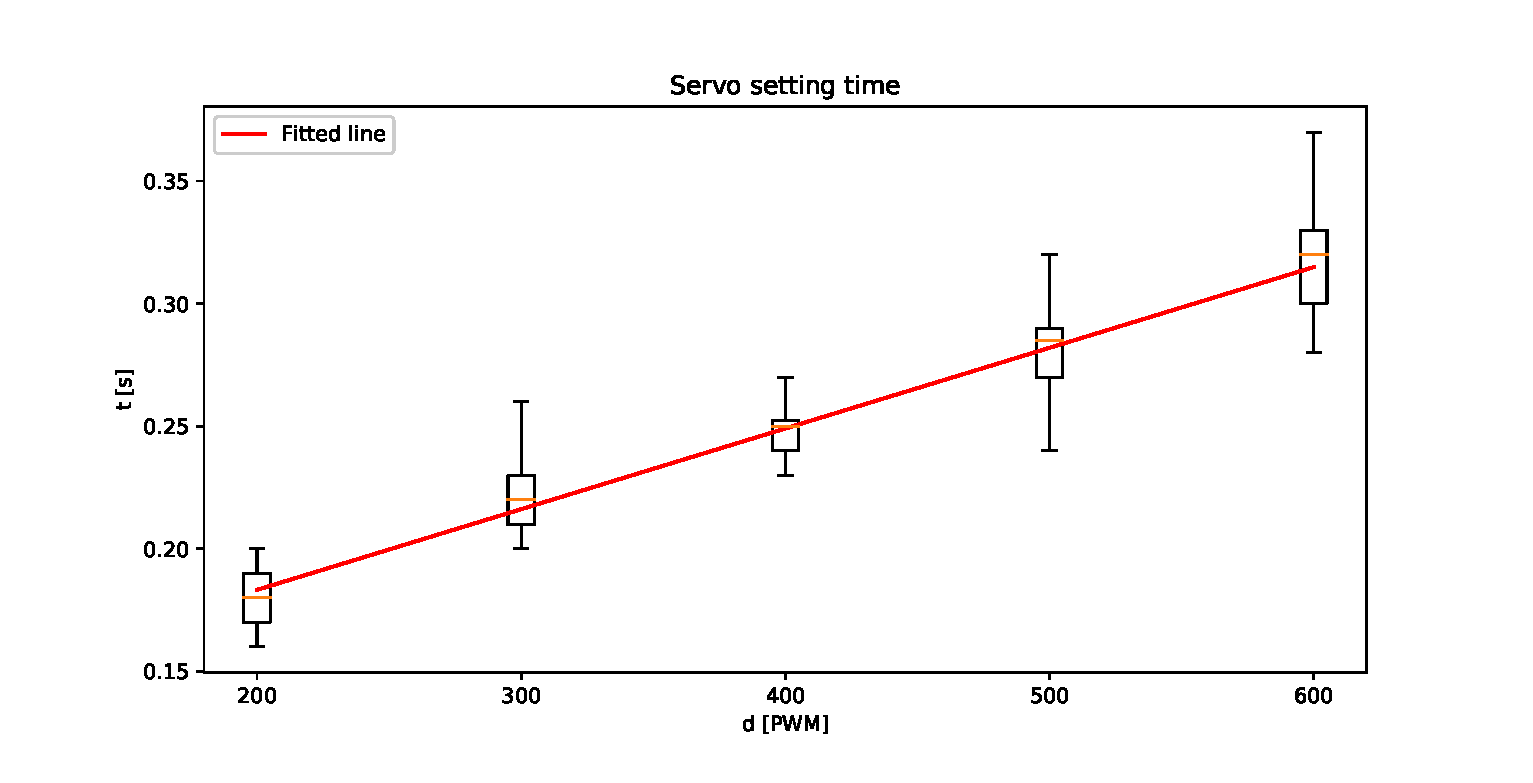
\includegraphics[width=\textwidth]{../img/servo_setting_time_linreg.eps}
	\caption{The setting time of the steering servo can be estimated with a linear function of the distance between the start and end PWM values.}
	\label{fig:servo_linear_regression}
\end{figure}

\section{Motor Shaft Angular Velocity Modeling}
\chapter*{Conclusion}
\addcontentsline{toc}{chapter}{Conclusion}

In this thesis, we approached the problem of autonomous racing inspired by the F1/10 competition. This problem is a simplification of full-scale autonomous vehicle driving which allowed us to focus solely on collision-free time-optimal car-like vehicle motion without having to take into account other intricacies of the adjacent problems, such as obeying traffic rules and predicting the behavior of other road users and pedestrians.

Our approach to solve the problem was to create an agent, which analyzes the layout of the racing circuit and then plans its motion through the track focusing on just a fixed number of corners ahead of the vehicle. Using the Hybrid A* and the \gls{SEHS} algorithms, we were able to generate nearly time-optimal trajectories as the vehicle drives along the racing circuit in almost real-time. Our planning algorithm was able to consider stationary obstacles which were discovered using the sensors of the vehicle in previous laps.

We implemented two trajectory following strategies – the Pure Pursuit controller and the \gls{DWA} algorithm. Both algorithms enabled the vehicle to move along the planned trajectory, both with their own advantages. The Pure Pursuit algorithm follows the planned trajectory closely, but it follows it blindly and it does not avoid any unexpected obstacles. The \gls*{DWA} algorithm achieves similar comparable results and fast lap times and at the same time it allows the vehicle to avoid any obstacles which are detected as the vehicle moves and which were not considered by the planning algorithm.

We tested our algorithms on a car-like robot we built ourselves similarly to the F1/10 racing platform and on top of the \gls{ROS} ecosystem of tools and libraries. Although the planning algorithm performed sufficiently even with limited computation power, this test was not a success. Due to unreliable state estimation caused by the limited capabilities of the sensors, we were able to reach only very limited speeds at which we were able to move around the circuit. At higher speeds the vehicle would quickly lose track of its correct location and it would crash into a wall. When we eliminated the noisy data from the sensors and moved to a simulated environment, the vehicle was able to reach much higher speeds and reliably complete several laps of the circuit in a row.
nd Hybrid A* algorithms.

The experiments we conducted in a simulator show that our approach is viable. We are able to plan trajectories for the next three corners ahead of the vehicle at a frequency of several hertz and achieve good results on a test circuit. The vehicle also has a basic ability to detect and avoid unexpected obstacles. The most obvious shortcoming is the imprecise kinematic vehicle model. If we were able to predict the movement of the vehicle more reliably, the trajectories the planning algorithm produces would be easier to track and we would be able to navigate the vehicle through corners more safely without hitting the outer boundary of a corner. We could achieve further improvements by tuning the discretization parameters of the algorithms and the parameters and weights of the Pure Pursuit and DWA algorithms. It would be interesting to try the planning algorithm for a different F1/10 vehicle with reliable odometry and with identified parameters of a tire model. Since our code uses the standard \gls*{ROS} topic types and the standard transformation tree, the adaptation of our \gls*{ROS} nodes should be possible.

%%% Bibliography
\include{bibliography}

%%% Figures used in the thesis (consider if this is needed)
% \listoffigures

%%% Tables used in the thesis (consider if this is needed)
%%% In mathematical theses, it could be better to move the list of tables to the beginning of the thesis.
% \listoftables

\printglossaries

%%% Abbreviations used in the thesis, if any, including their explanation
%%% In mathematical theses, it could be better to move the list of abbreviations to the beginning of the thesis.
% \chapwithtoc{List of Abbreviations}

%%% Attachments to the master thesis, if any. Each attachment must be
%%% referred to at least once from the text of the thesis. Attachments
%%% are numbered.
%%%
%%% The printed version should preferably contain attachments, which can be
%%% read (additional tables and charts, supplementary text, examples of
%%% program output, etc.). The electronic version is more suited for attachments
%%% which will likely be used in an electronic form rather than read (program
%%% source code, data files, interactive charts, etc.). Electronic attachments
%%% should be uploaded to SIS and optionally also included in the thesis on a~CD/DVD.
%%% Allowed file formats are specified in provision of the rector no. 72/2017.
\appendix

\chapter{Experimental Vehicle}

\label{chapter:hardware}

In order to verify the approach we discuss in this theses, we needed a car-like robot which we could use for real-world testing. We took inspiration from the F1/10 competition \cite{F1/10}, the MIT RACECAR\footnote{\url{https://mit-racecar.github.io/}}, AutoRally\footnote{\url{https://autorally.github.io/}}, and other similar projects and we built a robot based on a chassis from an 1:10 scale \gls{RC} car with an on-board computer and a set of sensors. In this chapter, we will describe the hardware components we used to build a custom experimental fast moving car.

\section{Chassis}
\label{sec:chassis}

We used chassis, steering servo, \gls{DC} motor, \gls{ESC}, and a ratio transmitter and receiver from an off-the-shelf \gls*{RC} car. We removed the plastic cover and some unnecessary parts attached to the chassis and we attached a thin plywood board on top of the chassis. We later mounted all of the electronics to the plywood board. Even though the weight of the battery and of the electronics is not negligible, the suspension of the vehicle is stiff enough to carry the weight without any significant roll and pitch changes during acceleration and cornering.

\begin{figure}[!tbp]%
	\centering
	\begin{subfigure}[t]{0.45\textwidth}
		\includegraphics[width=\textwidth]{../img/car_top_no_electronics}
		\label{fig:chassis_no_electronics}
		\caption{A photo of the chassis of the vehicle without any additional electronics mounted to it.}
	\end{subfigure}
	\hfill
	\begin{subfigure}[t]{0.45\textwidth}
		\includegraphics[width=\textwidth]{../img/car_top}
		\label{fig:chassis_with_electronics}
		\caption{A photo of the chassis with the plywood board with all of the electronics attached to it. Some of the components are not visible  because they are attached to the bottom side of the board.}
	\end{subfigure}

	\vspace{1cm}

	\begin{subfigure}[b]{0.7\textwidth}		
		\includegraphics[width=\textwidth]{../img/car_front}
		\label{fig:chassis_front_view}
		\caption{Front view.}
	\end{subfigure}
	
	\caption{Photos of the experimental vehicle.}
	\label{fig:chassis}
\end{figure}

The chassis has the same geometry as a common passenger car with two fixed rear wheels and two front wheels with Ackermann steering geometry. All of the wheels are driven by the \gls*{DC} motor through a fixed gearbox. The wheels on both front and rear axes can move independently thanks to two differentials, one on each axis. The differentials are necessary for smooth travel during turns, when the outer wheel spins faster than the inner wheel. Photos of the vehicle are shown in Figure~\ref{fig:chassis} and the our measurements of the chassis are stated in Table~\ref{table:dimensions}.

\begin{table}
	\centering
	\begin{tabular}{l c r}
		\toprule
		Property name & Symbol & Measured value \\
		\midrule
		
		Wheelbase & $L$ & \SI{0.31}{\meter} \\
		Center of gravity offset & $l_r, l_f$ & \SI{0.155}{\meter} \\
		Width & $W$ & \SI{0.3}{\meter} \\
		Length & $H$ & \SI{0.45}{\meter} \\
		Wheel radius & $r_w$ & \SI{0.05}{\meter} \\
		Gear ratio (motor to wheels) & $G$ & \num{9} \\
		Reachable steering angles & $\delta$ & $\left[\ang{-21.16}, \ang{26.57}\right]$ \\
		\bottomrule
	\end{tabular}
	\caption{Properties of the chassis of the experimental vehicle.}
	\label{table:dimensions}
\end{table}

The steering servo and the \gls*{ESC}, which controls the speed of the \gls*{DC} motor, both have a 3-pin connector which was originally connected to a radio receiver. Two of the pins connect to a \gls*{DC} power supply and the third connects to a signal wire. The signal is originally created by an radio transmitter which generates a \gls{PWM} signal. The \gls*{PWM} signal consists of pattern resembling a square wave, where the voltage measured on the signal wire is high (\SI{5}{\volt}) for some period of time and then the voltage drops to low (\SI{0}{\volt}) for the rest of the period. The pulse of high voltage lasts between \SI{1}{\milli\second} and \SI{2}{\milli\second} and the period of the signal is \SI{20}{\milli\second} as it is shown in Figure~\ref{fig:pwm}. We can therefore connect these connectors to a computer which generates appropriate signals to steer the vehicle. The \SI{20}{\milli\second} period of one \gls*{PWM} cycle gives us an upper limit of \SI{50}{\hertz} at which we can change the commands for the vehicle.

\begin{figure}\centering
	\includegraphics[width=125mm]{../img/pwm.pdf}
	\caption{The PWM signal for the steering servo and the ESC form a square wave with the period of \SI{20}{\milli\second} and pulse width between \SIlist{1;2}{\milli\second}.}
	\label{fig:pwm}
\end{figure}

\section{Sensors}

The vehicle uses on-board sensors to track its location on the racing track. We use a combination of three sensors: a \gls{LIDAR}, an \gls{IMU}, and a motor encoder. We tried several different sensors from different manufacturers, including \verb|Razor 9DoF IMU| and \verb|Scanse Sweep 2D LIDAR|, but these devices did not yield good results. 

\paragraph{Hall Effect Encoder} consists of an 8-pole magnetic disc which we attach to the drive shaft of the vehicle, and a Hall effect sensor. The sensor sends a pulse every time it detects a change from a north pole to a south pole or vice-versa. This way we can detect that the motor has made one eigth of a revolution. By counting the number of revolutions and by assuming that the wheels of the vehicle roll perfectly against the road surface, we can estimate the distance that the vehicle traveled. By combining this information with the current steering angle of the front wheels, we can estimate the movement of the vehicle and use it as a source of odometry. We used a ``Wheel Encoder Kit from DAGU'' from SparkFun\footnote{\url{https://www.sparkfun.com/products/12629}}.

\paragraph{Bosch BNO055 USB Stick} is an \gls{IMU} which contains a triaxial accelerometer, a triaxial gyroscope, a triaxial magnetometer and a thermometer\footnote{\url{https://www.bosch-sensortec.com/bst/products/all\_products/bno055}}. We use the measurements of the gyroscope and the accelerometer to determine the acceleration of the vehicle to improve our odometry from the motor encoder, which cannot detect wheel skidding.

\paragraph{YDLIDAR X4} is a low-cost \ang{360} \gls{LIDAR} laser scanner. We use it to determine the distance to the surrounding obstacles. This sensor has a range of up to \SI{10}{\meter} and it takes \num{5000} samples every second while spinning at the frequency of almost \SI{12}{\hertz}. This sensor is connected to a computer via a micro-USB port and it is connected to a \SI{5}{\volt} power supply through a second micro-USB port.

\section{On-board Computer}

The brains of our autonomous vehicle is the NVIDIA Jetson Nano\footnote{\url{https://developer.nvidia.com/embedded/jetson-nano-developer-kit}}. This board contains a quad-core ARM A57 with the clock frequency of \SI{1.43}{\giga\hertz}, \SI{4}{\giga B} of LPDDR4 RAM and a 128-core Maxwell GPU. This computer is powered through a Micro-USB port with \SI{5}{\volt}/\SI{2}{\ampere}\footnote{The board can operate with a lower power consumption of \SI{5}{\watt} in a mode in which two of the CPU cores are turned off.}. The Jetson has 4 USB ports which are used to connect the \gls*{LIDAR}, the \gls*{IMU}, and two Arduino boards. The board does not include a Wi-Fi antena and therefore we added an Intel Dual Band Wireless-Ac 8265 W/Bt card to the M.2 slot of the board in order to receive telemetry while the vehicle is driving along a circuit.

\subsection{Microcontrollers}

We use two Arduino Nano boards\footnote{\url{https://www.arduino.cc/en/Guide/ArduinoNano}} as an interface between the actuators, the radio receiver, and the motor encoder, and the Jetson Nano board.

\paragraph{Hall Effect Encoder} is connected to an interrupt pin of one Arduino and this Arduino counts the number of revolutions of the motor. This board also provides power to the Hall sensor.

\paragraph{ESC and Servo} are connected to \gls{PWM} output pins of the other Arduino board and the radio receiver is connected to two interrupt pins. This board contains logic which converts high-level commands for the actuators into corresponding \gls*{PWM} signals. It also contains a safety mechanism which disables autonomous mode of the vehicle and allows the supervisor to take over control of the vehicle when he or she uses the remote controller.

\section{Power Supply}

The \gls*{DC} motor and the servo are powered by \SI{7.2}{\volt} \SI{5000}{\milli\ampere\hour} NiMH battery which was included with the \gls*{RC} car. The rest of the electronics of the vehicle is powered by a regular \SI{20000}{\milli\ampere\hour} power bank which has two output USB ports. One of these ports can supply \SI{2}{\ampere} and the Jetson Nano board is connected to it, the other port can supply \SI{1}{\ampere} and it powers the \gls*{LIDAR}.

This setup ensures that the power in the batteries supplying the motors of the vehicle discharge much sooner than the power bank which supplies the computer and sensors if we start with fully charged batteries. It should never occur that the computer shuts down while the car is being driven autonomously and it will not continue moving uncontrollably. We also do not need to build a custom power delivery board.

\chapter{Programmer Documentation}

The implementation of our autonomous racing agent relies on a complex set of libraries and tools. In this chapter, we will describe the libraries and tools we used and we will briefly explain how some of them work. We will also explain how we implemented the behavior of the autonomous racing agent in the context of this setup. The installation instructions and instructions on how to deploy and use the software used and developed in this thesis are covered in the following chapter \ref{chapter:user_documentation}.

\section{Robot Operating System}

Robot Operating System (ROS) is an open-source set of libraries and tools built on top of Linux. Processes running under this operating system are referred to as nodes and they can be distributed across multiple computers connected over a wired or wireless network or through a serial port. Nodes can be programmed in many different programming languages but the most common and officially supported languages are Python and C++.

Nodes communicate between each other using a publisher/subscriber pattern. A node can advertise any number of topics through which it publishes its outputs in a form of messages. It can also subscribe to topics advertised by other nodes and it can work with the received messages as its outputs. This way it is possible to create a complex system by combining many small and simple specialized nodes.

Each topic has an assigned message type which defines the structure of the data. There is a large number of standard messages which are used by authors of public libraries. This way it is often possible to replace one library with a different one without additional changes to other nodes. This can be useful for example when one sensor is replaced by a device of the same type but from a different vendor whose ROS node publishes the same standard message type. Programmers can also define their custom message types which are better suited for their application.

ROS comes with a variety of tools for debugging and visualization of the data passed through the topics. One of these tools is Rviz. It is a convenient way of visualizing the current state of the system. We use this tool to visualize the telemetry data from the vehicle on a laptop while it is driving along the racing circuit.

We use the ROS release named ``Melodic Morenia'' which is compatible with Ubuntu 18.04 LTS. Further information about ROS and tutorials which describe how to work with it are available on the official website of the ROS project\footnote{https://www.ros.org}.

\section{Architecture Of The Distributed System}

The setup of our robot consists of the NVIDIA Jetson Nano board which is mounted on the vehicle, two Arduinos which are connected to the Jetson through a serial port, and a notebook which is connected to Jetson over Wi-Fi. Jetson acts as a ROS master machine, Arduinos act as an interface between Jetson and low-level hardware, and the notebook is used only to monitor telemetry data. The graph of this architecture and the connected sensors is depicted in Figure~\ref{fig:ros_diagram}.

\begin{figure}
	\centering
	\includegraphics[width=125mm]{../img/ros_diagram}
	\caption{This figure shows how the computers and sensors which make up the experimental vehicle are connected with each other and the direction of data flow between the devices.}
	\label{fig:rosdiagram}
\end{figure}

The communication between Arduino boards and the Jetson computer over USB is possible thanks to the \verb|rosserial| protocol\footnote{http://wiki.ros.org/rosserial}. Arduino microcontrollers use a \verb|ros_lib| library which allows us to subscribe to topics and to publish messages form the Arduino. On Jetson, the communication on each serial port is handled by an instance of a \verb|rosserial_python| node.

Each of the sensors connected through USB uses their own drivers for communication over the serial link. Luckily, open-source ROS packages for both the LIDAR and the IMU are available and both of them publish the data in the form of standard \verb|sensor_msgs/LaserScan|\footnote{http://docs.ros.org/melodic/api/sensor\_msgs/html/msg/LaserScan.html} and \verb|sensor_msgs/Imu|\footnote{http://docs.ros.org/melodic/api/sensor\_msgs/html/msg/Imu.html} messages. The data from the motor shaft encoder is published in the form of \verb|std_msgs/Float64| message and it contains the number of revolutions since the Arduino was last powered or reset.

The vehicle performs two tasks: mapping and racing. In the mapping phase the vehicle creates a map of the track using the LIDAR and in the racing phase it drives autonomously around the track with the knowledge of to the map and the topology of the circuit. In the following sections we will describe how we approach these two tasks.

\subsection{Mapping}

When the vehicle is creating the map of the track, it is being controlled manually using the remote controller of the vehicle. The only sensor which is needed for this task is the LIDAR. The data from the LIDAR is being collected by a SLAM algorithm (Simultaneous Localization And Mapping) implemeted by the Hector SLAM library by a tema from the Technical University of Darmstadt.

This library performs scan matching of the LIDAR scans and it builds a 2D occupancy grid of the environment over time. For an already built part of the map and a LIDAR scan consisting of $n$ points, the task of the scan matching algorithm is to find a rigid transformation $\xi =\left( p_x, p_y, \phi\right)$, which gives best alignment with the already built map. The authors formulate this problem as an optimization problem for solving in \cite{HectorSlam}:

$$
\xi^* = \underset{\xi}{\arg\min} \sum_{i=1}^n\left[ 1 - M\left( S_i\left( \xi\right)\right)\right]^2,
$$

where $S_i\left(\xi\right)$ are the world coordinates of scan point $s_i$ after applying the transform $\xi$ and the function $M$ gives the value of the occupancy grid at the given coordinates.

Hector SLAM provides a ROS node \verb|hector_mapping| which subscribes to a topic providing \verb|sensor_msgs/LaserScan|\footnote{http://docs.ros.org/melodic/api/sensor\_msgs/html/msg/LaserScan.html} messages and publishes its output in a topic of type \verb|nav_msgs/OccupancyGrid|\footnote{http://docs.ros.org/melodic/api/nav\_msgs/html/msg/OccupancyGrid.html}. When the mapping is complete, the final map can be saved into a file using a \verb|map_saver| node from the \verb|map_server| package\footnote{http://wiki.ros.org/map\_server\#map\_saver}.

\subsection{Racing}

The inputs for the racing task are the map of the track in the form of an occupancy grid, and a list of coordinates in the map representing the checkpoints defining the topology of the racing circuit. This is significantly more complicated than the mapping task and the implementation is split into three groups of ROS nodes: odometry and localization, agent behavior, and a hardware interface.

\subsubsection{Odometry and Localization}

Odometry is an estimate of how position of the robot changes over time based on data from sensors which measure the movement of the robot. Odometry is supposed to be continuous and there should not be any sudden changes in the position of the vehicle. The data from the sensors is inherently noisy and inaccurate and the estimated position of the robot will become more and more inaccurate over time. This phenomenon is referred to as drift.

To counteract the drift, we perform a correction using the AMCL (Adaptive Monte Carlo Localization) algorithm. This algorithm uses the data from the LIDAR to determine the position of the vehicle in the map based on the distances to the obstacles around it. Unlike odometry, the sequence of position updates is not expected to be continuous and the resulting location can in theory be a point anywhere on the map.

Our vehicle has two sources of odometry: the number of revolutions of the motor shaft and the accelerations measured by the IMU. We implemented a simple ROS node which subscribes to the motor shaft encoder and the steering commands supplied to the vehicle. From the number of revolutions and an assumption that the wheels are not skidding we can estimate the distance the vehicle travelled since the last update. From the steering command, we can estimate the steering angle of the front wheels of the vehicle. From these two inputs, we can estimate how the vehicle body translated and rotated using a simple kinematic vehicle model. This approach was inspired by the MIT RACECAR VESC odometry ROS node\footnote{https://github.com/mit-racecar/vesc}. These sources are then fused into a pose estimate using the \verb|robot_pose_ekf| node\footnote{https://wiki.ros.org/robot\_pose\_ekf}. This node uses EKF (Extended Kalman Filter) to estimate the most likely location from the input sources and their covariances. We also tried to use a newer ROS package \verb|robot_localization| which also implements an EKF, but the results were less accurate.



\chapter{Attachments}
\label{chapter:user_documentation}

\todo[inline]{Give some brief introduction and set the expectations.}

\section{Trajectory Planning And Track Analysis Algorithms}

In order to test the \gls{SEHS} and Hybrid A* track analysis algorithm from Section~\ref{sec:track_segmentation} and the \gls{SEHS} and Hybrid A* trajectory planning algorithms described in Chapter~\ref{chapter:trajectory_planning}, we wrote two C++ programs to test these algorithms on different inputs and to visualize their outcomes.

\subsection{Requirements and Compilation}

In order to compile and run these test programs, we recommend using a PC running a Linux distribution. Both programs were also successfully tested on Microsoft Windows 10 with \textit{Windows Subsystem for Linux} (WSL) 2 and the \textit{X Window System}, such as \textit{Xming X Server}\footnote{\url{http://www.straightrunning.com/XmingNotes/}}, installed. The programs are written using C++17 and they are meant to be compiled using the G++ 9.2 compiler\footnote{\url{https://gcc.gnu.org/gcc-9/}}.

To visualize the outputs of the algorithms, we use the \textit{Matplotib} library and its C++ binding library \texttt{matplotlib-cpp}. The source code of this library and other resources are available in a Git repository hosted at \url{https://github.com/lava/matplotlib-cpp}\footnote{At the time of writing, the latest version of the library had the checksum of \texttt{d612b524e10ebdd43d3a8889a95e84c017ad65af}. Our code might not be compatible with future revisions of the library.}. In order to set up this library, install the dependencies of the library first\footnote{The instructions are available at \url{https://github.com/lava/matplotlib-cpp/tree/d612b524e10ebdd43d3a8889a95e84c017ad65af#installation}.} and then clone the repository using the \textit{Git} tool\footnote{https://git-scm.com/} and change the repository to the version needed in our code:

\begin{lstlisting}
cd experiments/algorithm-testing/include
git clone https://github.com/lava/matplotlib-cpp
cd matplotlib-cpp
git checkout d612b524e10ebdd43d3a8889a95e84c017ad65af
\end{lstlisting}

To compile and link the source code into executable binaries, use the prepared \texttt{Makefile}:

\begin{lstlisting}
make -C experiments/algorithm-testing
\end{lstlisting}

The two binaries will be located in the \texttt{experiments/algorithm-testing/bin} directory.

\subsection{Usage}

\todo[inline]{Describe how to use both commands.}

\subsection{Circuit Definition File Format}

\todo[inline]{Describe the format of the file.}

\section{ROS Nodes}

\todo[inline]{Describe everything.}

\openright
\end{document}
